\documentclass[journal]{IEEEtran}
\usepackage[T1]{fontenc}
\usepackage{amsmath,amssymb,graphicx,booktabs,array,url,textcomp,siunitx}
\usepackage[hidelinks]{hyperref}
\sisetup{detect-all, per-mode=symbol, group-minimum-digits=4}
\newcolumntype{L}[1]{>{\raggedright\arraybackslash}p{#1}}
\graphicspath{{figs/}}
\newcommand{\du}{\Delta u_{\mathrm{c}}}
\newcommand{\deps}{\Delta\varepsilon_{\mathrm{in}}}
\IfFileExists{results_macros.tex}{% GENERATED by scripts/tcpmt_manuscript_macros.py -- do not edit
% source: /home/beams0/SABDELZAHER/ETM_project/HVR_OPT_work/research/final_closure
\newcommand{\PlossZone}{144.3}
\newcommand{\EffZone}{87.4}
\newcommand{\PconvZone}{140.7}
\newcommand{\ProuteZone}{3.62}
\newcommand{\PhvZone}{1.77}
\newcommand{\PtsvZone}{0.00}
\newcommand{\PattZone}{--}
\newcommand{\PintraZone}{1.81}
\newcommand{\PboardZone}{--}
\newcommand{\PpadsZone}{0.044}
\newcommand{\TmaxZone}{115.7}
\newcommand{\TdieZone}{89.8}
\newcommand{\TconvZone}{107.7}
\newcommand{\TjointZone}{115.0}
\newcommand{\WarpZone}{25.5}
\newcommand{\PkgWarpZone}{25.2}
\newcommand{\DuZone}{2.21}
\newcommand{\EpsZone}{5.71}
\newcommand{\EpsUZone}{1.7}
\newcommand{\EtItersZone}{5}
\newcommand{\TjointHotZone}{115.4}
\newcommand{\TlsZone}{109.7}
\newcommand{\TlsRiseZone}{85}
\newcommand{\ThsZone}{112.7}
\newcommand{\TindZone}{100.7}
\newcommand{\QplateZone}{--}
\newcommand{\QtopZone}{--}
\newcommand{\QdieDownZone}{--}
\newcommand{\NjointZone}{1369}
\newcommand{\PrtZone}{94.1}
\newcommand{\UnderZone}{35}
\newcommand{\RiseZone}{50.2}
\newcommand{\PlossZoneSone}{179.9}
\newcommand{\EffZoneSone}{84.7}
\newcommand{\PconvZoneSone}{144.8}
\newcommand{\ProuteZoneSone}{35.13}
\newcommand{\PhvZoneSone}{31.48}
\newcommand{\PtsvZoneSone}{0.01}
\newcommand{\PattZoneSone}{--}
\newcommand{\PintraZoneSone}{3.60}
\newcommand{\PboardZoneSone}{--}
\newcommand{\PpadsZoneSone}{0.045}
\newcommand{\TmaxZoneSone}{140.5}
\newcommand{\TdieZoneSone}{91.9}
\newcommand{\TconvZoneSone}{115.4}
\newcommand{\TjointZoneSone}{140.3}
\newcommand{\WarpZoneSone}{32.3}
\newcommand{\PkgWarpZoneSone}{32.6}
\newcommand{\DuZoneSone}{2.72}
\newcommand{\EpsZoneSone}{8.14}
\newcommand{\EpsUZoneSone}{1.1}
\newcommand{\EtItersZoneSone}{5}
\newcommand{\TjointHotZoneSone}{140.3}
\newcommand{\TlsZoneSone}{116.7}
\newcommand{\TlsRiseZoneSone}{92}
\newcommand{\ThsZoneSone}{123.3}
\newcommand{\TindZoneSone}{105.2}
\newcommand{\QplateZoneSone}{--}
\newcommand{\QtopZoneSone}{--}
\newcommand{\QdieDownZoneSone}{--}
\newcommand{\NjointZoneSone}{1369}
\newcommand{\PrtZoneSone}{114.2}
\newcommand{\UnderZoneSone}{37}
\newcommand{\RiseZoneSone}{65.7}
\newcommand{\PlossZoneStwo}{296.6}
\newcommand{\EffZoneStwo}{77.1}
\newcommand{\PconvZoneStwo}{158.4}
\newcommand{\ProuteZoneStwo}{138.22}
\newcommand{\PhvZoneStwo}{130.28}
\newcommand{\PtsvZoneStwo}{0.02}
\newcommand{\PattZoneStwo}{--}
\newcommand{\PintraZoneStwo}{7.87}
\newcommand{\PboardZoneStwo}{--}
\newcommand{\PpadsZoneStwo}{0.046}
\newcommand{\TmaxZoneStwo}{225.1}
\newcommand{\TdieZoneStwo}{98.6}
\newcommand{\TconvZoneStwo}{140.7}
\newcommand{\TjointZoneStwo}{224.3}
\newcommand{\WarpZoneStwo}{54.7}
\newcommand{\PkgWarpZoneStwo}{57.0}
\newcommand{\DuZoneStwo}{4.41}
\newcommand{\EpsZoneStwo}{--}
\newcommand{\EpsUZoneStwo}{--}
\newcommand{\EtItersZoneStwo}{7}
\newcommand{\TjointHotZoneStwo}{224.3}
\newcommand{\TlsZoneStwo}{139.6}
\newcommand{\TlsRiseZoneStwo}{115}
\newcommand{\ThsZoneStwo}{158.3}
\newcommand{\TindZoneStwo}{120.0}
\newcommand{\QplateZoneStwo}{--}
\newcommand{\QtopZoneStwo}{--}
\newcommand{\QdieDownZoneStwo}{--}
\newcommand{\NjointZoneStwo}{1369}
\newcommand{\PrtZoneStwo}{162.5}
\newcommand{\UnderZoneStwo}{45}
\newcommand{\RiseZoneStwo}{134.1}
\newcommand{\PlossZtwo}{147.4}
\newcommand{\EffZtwo}{87.2}
\newcommand{\PconvZtwo}{144.8}
\newcommand{\ProuteZtwo}{2.67}
\newcommand{\PhvZtwo}{--}
\newcommand{\PtsvZtwo}{0.55}
\newcommand{\PattZtwo}{0.23}
\newcommand{\PintraZtwo}{1.84}
\newcommand{\PboardZtwo}{--}
\newcommand{\PpadsZtwo}{0.044}
\newcommand{\TmaxZtwo}{124.3}
\newcommand{\TdieZtwo}{90.0}
\newcommand{\TconvZtwo}{113.6}
\newcommand{\TjointZtwo}{97.2}
\newcommand{\WarpZtwo}{68.7}
\newcommand{\PkgWarpZtwo}{102.7}
\newcommand{\DuZtwo}{3.09}
\newcommand{\EpsZtwo}{7.85}
\newcommand{\EpsUZtwo}{0.8}
\newcommand{\EtItersZtwo}{5}
\newcommand{\TjointHotZtwo}{98.3}
\newcommand{\TlsZtwo}{116.7}
\newcommand{\TlsRiseZtwo}{92}
\newcommand{\ThsZtwo}{119.7}
\newcommand{\TindZtwo}{107.1}
\newcommand{\QplateZtwo}{--}
\newcommand{\QtopZtwo}{--}
\newcommand{\QdieDownZtwo}{--}
\newcommand{\NjointZtwo}{528}
\newcommand{\PrtZtwo}{93.5}
\newcommand{\UnderZtwo}{37}
\newcommand{\RiseZtwo}{54.0}
\newcommand{\PlossZtwoSone}{149.4}
\newcommand{\EffZtwoSone}{87.0}
\newcommand{\PconvZtwoSone}{145.0}
\newcommand{\ProuteZtwoSone}{4.42}
\newcommand{\PhvZtwoSone}{--}
\newcommand{\PtsvZtwoSone}{0.56}
\newcommand{\PattZtwoSone}{0.23}
\newcommand{\PintraZtwoSone}{3.59}
\newcommand{\PboardZtwoSone}{--}
\newcommand{\PpadsZtwoSone}{0.044}
\newcommand{\TmaxZtwoSone}{124.8}
\newcommand{\TdieZtwoSone}{90.1}
\newcommand{\TconvZtwoSone}{114.0}
\newcommand{\TjointZtwoSone}{97.4}
\newcommand{\WarpZtwoSone}{69.0}
\newcommand{\PkgWarpZtwoSone}{103.1}
\newcommand{\DuZtwoSone}{3.10}
\newcommand{\EpsZtwoSone}{7.88}
\newcommand{\EpsUZtwoSone}{0.8}
\newcommand{\EtItersZtwoSone}{5}
\newcommand{\TjointHotZtwoSone}{98.4}
\newcommand{\TlsZtwoSone}{117.2}
\newcommand{\TlsRiseZtwoSone}{92}
\newcommand{\ThsZtwoSone}{120.2}
\newcommand{\TindZtwoSone}{107.5}
\newcommand{\QplateZtwoSone}{--}
\newcommand{\QtopZtwoSone}{--}
\newcommand{\QdieDownZtwoSone}{--}
\newcommand{\NjointZtwoSone}{528}
\newcommand{\PrtZtwoSone}{94.8}
\newcommand{\UnderZtwoSone}{37}
\newcommand{\RiseZtwoSone}{54.7}
\newcommand{\PlossZtwoStwo}{153.7}
\newcommand{\EffZtwoStwo}{86.7}
\newcommand{\PconvZtwoStwo}{145.5}
\newcommand{\ProuteZtwoStwo}{8.16}
\newcommand{\PhvZtwoStwo}{--}
\newcommand{\PtsvZtwoStwo}{0.56}
\newcommand{\PattZtwoStwo}{0.23}
\newcommand{\PintraZtwoStwo}{7.33}
\newcommand{\PboardZtwoStwo}{--}
\newcommand{\PpadsZtwoStwo}{0.044}
\newcommand{\TmaxZtwoStwo}{125.9}
\newcommand{\TdieZtwoStwo}{90.3}
\newcommand{\TconvZtwoStwo}{114.9}
\newcommand{\TjointZtwoStwo}{97.7}
\newcommand{\WarpZtwoStwo}{69.7}
\newcommand{\PkgWarpZtwoStwo}{104.0}
\newcommand{\DuZtwoStwo}{3.11}
\newcommand{\EpsZtwoStwo}{7.95}
\newcommand{\EpsUZtwoStwo}{0.8}
\newcommand{\EtItersZtwoStwo}{5}
\newcommand{\TjointHotZtwoStwo}{98.8}
\newcommand{\TlsZtwoStwo}{118.1}
\newcommand{\TlsRiseZtwoStwo}{93}
\newcommand{\ThsZtwoStwo}{121.2}
\newcommand{\TindZtwoStwo}{108.1}
\newcommand{\QplateZtwoStwo}{--}
\newcommand{\QtopZtwoStwo}{--}
\newcommand{\QdieDownZtwoStwo}{--}
\newcommand{\NjointZtwoStwo}{528}
\newcommand{\PrtZtwoStwo}{97.5}
\newcommand{\UnderZtwoStwo}{37}
\newcommand{\RiseZtwoStwo}{56.1}
\newcommand{\PlossZthree}{120.3}
\newcommand{\EffZthree}{89.3}
\newcommand{\PconvZthree}{105.7}
\newcommand{\ProuteZthree}{14.63}
\newcommand{\PhvZthree}{--}
\newcommand{\PtsvZthree}{0.52}
\newcommand{\PattZthree}{2.29}
\newcommand{\PintraZthree}{1.48}
\newcommand{\PboardZthree}{10.29}
\newcommand{\PpadsZthree}{0.043}
\newcommand{\TmaxZthree}{82.4}
\newcommand{\TdieZthree}{78.5}
\newcommand{\TconvZthree}{45.9}
\newcommand{\TjointZthree}{78.7}
\newcommand{\WarpZthree}{4.7}
\newcommand{\PkgWarpZthree}{13.9}
\newcommand{\DuZthree}{1.41}
\newcommand{\EpsZthree}{1.98}
\newcommand{\EpsUZthree}{12.1}
\newcommand{\EtItersZthree}{4}
\newcommand{\TjointHotZthree}{79.2}
\newcommand{\TlsZthree}{50.3}
\newcommand{\TlsRiseZthree}{25}
\newcommand{\ThsZthree}{31.3}
\newcommand{\TindZthree}{56.3}
\newcommand{\QplateZthree}{173}
\newcommand{\QtopZthree}{947}
\newcommand{\QdieDownZthree}{53}
\newcommand{\NjointZthree}{1369}
\newcommand{\PrtZthree}{104.1}
\newcommand{\UnderZthree}{13}
\newcommand{\RiseZthree}{16.2}
\newcommand{\PlossZthreeSone}{121.8}
\newcommand{\EffZthreeSone}{89.1}
\newcommand{\PconvZthreeSone}{105.8}
\newcommand{\ProuteZthreeSone}{16.04}
\newcommand{\PhvZthreeSone}{--}
\newcommand{\PtsvZthreeSone}{0.52}
\newcommand{\PattZthreeSone}{2.29}
\newcommand{\PintraZthreeSone}{2.89}
\newcommand{\PboardZthreeSone}{10.29}
\newcommand{\PpadsZthreeSone}{0.043}
\newcommand{\TmaxZthreeSone}{82.5}
\newcommand{\TdieZthreeSone}{78.5}
\newcommand{\TconvZthreeSone}{46.0}
\newcommand{\TjointZthreeSone}{78.8}
\newcommand{\WarpZthreeSone}{4.8}
\newcommand{\PkgWarpZthreeSone}{14.0}
\newcommand{\DuZthreeSone}{1.41}
\newcommand{\EpsZthreeSone}{1.99}
\newcommand{\EpsUZthreeSone}{12.0}
\newcommand{\EtItersZthreeSone}{4}
\newcommand{\TjointHotZthreeSone}{79.2}
\newcommand{\TlsZthreeSone}{50.4}
\newcommand{\TlsRiseZthreeSone}{25}
\newcommand{\ThsZthreeSone}{31.3}
\newcommand{\TindZthreeSone}{56.4}
\newcommand{\QplateZthreeSone}{174}
\newcommand{\QtopZthreeSone}{948}
\newcommand{\QdieDownZthreeSone}{52}
\newcommand{\NjointZthreeSone}{1369}
\newcommand{\PrtZthreeSone}{105.4}
\newcommand{\UnderZthreeSone}{13}
\newcommand{\RiseZthreeSone}{16.4}
\newcommand{\PlossZthreeStwo}{125.0}
\newcommand{\EffZthreeStwo}{88.9}
\newcommand{\PconvZthreeStwo}{105.9}
\newcommand{\ProuteZthreeStwo}{19.05}
\newcommand{\PhvZthreeStwo}{--}
\newcommand{\PtsvZthreeStwo}{0.52}
\newcommand{\PattZthreeStwo}{2.30}
\newcommand{\PintraZthreeStwo}{5.89}
\newcommand{\PboardZthreeStwo}{10.30}
\newcommand{\PpadsZthreeStwo}{0.043}
\newcommand{\TmaxZthreeStwo}{82.5}
\newcommand{\TdieZthreeStwo}{78.6}
\newcommand{\TconvZthreeStwo}{46.3}
\newcommand{\TjointZthreeStwo}{78.9}
\newcommand{\WarpZthreeStwo}{4.9}
\newcommand{\PkgWarpZthreeStwo}{14.2}
\newcommand{\DuZthreeStwo}{1.42}
\newcommand{\EpsZthreeStwo}{2.02}
\newcommand{\EpsUZthreeStwo}{11.8}
\newcommand{\EtItersZthreeStwo}{4}
\newcommand{\TjointHotZthreeStwo}{79.3}
\newcommand{\TlsZthreeStwo}{50.7}
\newcommand{\TlsRiseZthreeStwo}{26}
\newcommand{\ThsZthreeStwo}{31.4}
\newcommand{\TindZthreeStwo}{56.7}
\newcommand{\QplateZthreeStwo}{176}
\newcommand{\QtopZthreeStwo}{948}
\newcommand{\QdieDownZthreeStwo}{51}
\newcommand{\NjointZthreeStwo}{1369}
\newcommand{\PrtZthreeStwo}{108.2}
\newcommand{\UnderZthreeStwo}{13}
\newcommand{\RiseZthreeStwo}{16.8}
\newcommand{\DeltaPZtwoSzero}{-3.13}
\newcommand{\DeltaPrtZtwoSzero}{0.59}
\newcommand{\DeltaPrtAbsZtwoSzero}{0.6}
\newcommand{\DeltaPZthreeSzero}{23.99}
\newcommand{\DeltaPrtZthreeSzero}{-10.02}
\newcommand{\DeltaPrtAbsZthreeSzero}{10.0}
\newcommand{\DeltaPZtwoSone}{30.51}
\newcommand{\DeltaPrtZtwoSone}{19.46}
\newcommand{\DeltaPrtAbsZtwoSone}{19.5}
\newcommand{\DeltaPZthreeSone}{58.13}
\newcommand{\DeltaPrtZthreeSone}{8.84}
\newcommand{\DeltaPrtAbsZthreeSone}{8.8}
\newcommand{\DeltaPZtwoStwo}{142.88}
\newcommand{\DeltaPrtZtwoStwo}{64.93}
\newcommand{\DeltaPrtAbsZtwoStwo}{64.9}
\newcommand{\DeltaPZthreeStwo}{171.59}
\newcommand{\DeltaPrtZthreeStwo}{54.32}
\newcommand{\DeltaPrtAbsZthreeStwo}{54.3}
\newcommand{\LossGapZtwoSzero}{3.1}
\newcommand{\LossLeadZtwoSzero}{Z1}
\newcommand{\dPconvZtwoSzero}{4.08}
\newcommand{\dPconvAbsZtwoSzero}{4.1}
\newcommand{\dProuteZtwoSzero}{-0.95}
\newcommand{\dProuteAbsZtwoSzero}{0.95}
\newcommand{\dTlsZtwoSzero}{7.0}
\newcommand{\dTlsAbsZtwoSzero}{7}
\newcommand{\dTmaxZtwoSzero}{8.7}
\newcommand{\dTmaxAbsZtwoSzero}{9}
\newcommand{\dTjointZtwoSzero}{-17.7}
\newcommand{\dTjointAbsZtwoSzero}{18}
\newcommand{\LossGapZthreeSzero}{24.0}
\newcommand{\LossLeadZthreeSzero}{Z3}
\newcommand{\dPconvZthreeSzero}{-34.99}
\newcommand{\dPconvAbsZthreeSzero}{35.0}
\newcommand{\dProuteZthreeSzero}{11.00}
\newcommand{\dProuteAbsZthreeSzero}{11.00}
\newcommand{\dTlsZthreeSzero}{-59.4}
\newcommand{\dTlsAbsZthreeSzero}{59}
\newcommand{\dTmaxZthreeSzero}{-33.2}
\newcommand{\dTmaxAbsZthreeSzero}{33}
\newcommand{\dTjointZthreeSzero}{-36.2}
\newcommand{\dTjointAbsZthreeSzero}{36}
\newcommand{\LossGapZtwoSone}{30.5}
\newcommand{\LossLeadZtwoSone}{Z2}
\newcommand{\dPconvZtwoSone}{0.20}
\newcommand{\dPconvAbsZtwoSone}{0.2}
\newcommand{\dProuteZtwoSone}{-30.71}
\newcommand{\dProuteAbsZtwoSone}{30.71}
\newcommand{\dTlsZtwoSone}{0.5}
\newcommand{\dTlsAbsZtwoSone}{0}
\newcommand{\dTmaxZtwoSone}{-15.7}
\newcommand{\dTmaxAbsZtwoSone}{16}
\newcommand{\dTjointZtwoSone}{-42.9}
\newcommand{\dTjointAbsZtwoSone}{43}
\newcommand{\LossGapZthreeSone}{58.1}
\newcommand{\LossLeadZthreeSone}{Z3}
\newcommand{\dPconvZthreeSone}{-39.04}
\newcommand{\dPconvAbsZthreeSone}{39.0}
\newcommand{\dProuteZthreeSone}{-19.09}
\newcommand{\dProuteAbsZthreeSone}{19.09}
\newcommand{\dTlsZthreeSone}{-66.3}
\newcommand{\dTlsAbsZthreeSone}{66}
\newcommand{\dTmaxZthreeSone}{-58.1}
\newcommand{\dTmaxAbsZthreeSone}{58}
\newcommand{\dTjointZthreeSone}{-61.5}
\newcommand{\dTjointAbsZthreeSone}{62}
\newcommand{\LossGapZtwoStwo}{142.9}
\newcommand{\LossLeadZtwoStwo}{Z2}
\newcommand{\dPconvZtwoStwo}{-12.83}
\newcommand{\dPconvAbsZtwoStwo}{12.8}
\newcommand{\dProuteZtwoStwo}{-130.05}
\newcommand{\dProuteAbsZtwoStwo}{130.05}
\newcommand{\dTlsZtwoStwo}{-21.6}
\newcommand{\dTlsAbsZtwoStwo}{22}
\newcommand{\dTmaxZtwoStwo}{-99.2}
\newcommand{\dTmaxAbsZtwoStwo}{99}
\newcommand{\dTjointZtwoStwo}{-126.5}
\newcommand{\dTjointAbsZtwoStwo}{127}
\newcommand{\LossGapZthreeStwo}{171.6}
\newcommand{\LossLeadZthreeStwo}{Z3}
\newcommand{\dPconvZthreeStwo}{-52.42}
\newcommand{\dPconvAbsZthreeStwo}{52.4}
\newcommand{\dProuteZthreeStwo}{-119.17}
\newcommand{\dProuteAbsZthreeStwo}{119.17}
\newcommand{\dTlsZthreeStwo}{-89.0}
\newcommand{\dTlsAbsZthreeStwo}{89}
\newcommand{\dTmaxZthreeStwo}{-142.6}
\newcommand{\dTmaxAbsZthreeStwo}{143}
\newcommand{\dTjointZthreeStwo}{-145.4}
\newcommand{\dTjointAbsZthreeStwo}{145}
\newcommand{\RiseSoneZone}{35.6}
\newcommand{\RiseSoneZtwo}{2.0}
\newcommand{\RiseSoneZthree}{1.5}
\newcommand{\ConvToRouteZtwo}{4.3}
\newcommand{\ConvToRouteZthree}{3.2}
\newcommand{\NvariantRuns}{57}
\newcommand{\WarpRatioZtwo}{2.69}
\newcommand{\WarpFoldZtwo}{0.4}
\newcommand{\DuRatioZtwo}{1.40}
\newcommand{\WarpRatioZthree}{0.19}
\newcommand{\WarpFoldZthree}{5.4}
\newcommand{\DuRatioZthree}{0.64}
\newcommand{\LandTie}{28}
\newcommand{\LandPT}{667}
\newcommand{\LandPmax}{67}
\newcommand{\LandTmin}{10}
\newcommand{\LandPmin}{11}
\newcommand{\LandTmax}{60}
\newcommand{\LandDVmax}{163}
\newcommand{\LandDVmin}{27}
\newcommand{\LandBallsInside}{245}
\newcommand{\LandBallsRail}{685}
\newcommand{\PitchMaxZthree}{0.58}
\newcommand{\SensTierRefZonePloss}{152.1}
\newcommand{\SensDTierRefZonePloss}{7.8}
\newcommand{\SensDAbsTierRefZonePloss}{7.8}
\newcommand{\SensTierRefZoneTmax}{128.3}
\newcommand{\SensDTierRefZoneTmax}{12.7}
\newcommand{\SensDAbsTierRefZoneTmax}{12.7}
\newcommand{\SensTierRefZoneTls}{123.3}
\newcommand{\SensDTierRefZoneTls}{13.6}
\newcommand{\SensDAbsTierRefZoneTls}{13.6}
\newcommand{\SensTierRefZoneWarp}{38.2}
\newcommand{\SensDTierRefZoneWarp}{12.7}
\newcommand{\SensDAbsTierRefZoneWarp}{12.7}
\newcommand{\SensTierRefZoneDu}{3.81}
\newcommand{\SensDTierRefZoneDu}{1.60}
\newcommand{\SensDAbsTierRefZoneDu}{1.60}
\newcommand{\SensTierRefZoneTjoint}{128.0}
\newcommand{\SensDTierRefZoneTjoint}{13.0}
\newcommand{\SensDAbsTierRefZoneTjoint}{13.0}
\newcommand{\SensZtwoCooledZtwoPloss}{111.6}
\newcommand{\SensDZtwoCooledZtwoPloss}{-35.9}
\newcommand{\SensDAbsZtwoCooledZtwoPloss}{35.9}
\newcommand{\SensZtwoCooledZtwoTmax}{80.1}
\newcommand{\SensDZtwoCooledZtwoTmax}{-44.3}
\newcommand{\SensDAbsZtwoCooledZtwoTmax}{44.3}
\newcommand{\SensZtwoCooledZtwoTls}{56.5}
\newcommand{\SensDZtwoCooledZtwoTls}{-60.2}
\newcommand{\SensDAbsZtwoCooledZtwoTls}{60.2}
\newcommand{\SensZtwoCooledZtwoWarp}{12.9}
\newcommand{\SensDZtwoCooledZtwoWarp}{-55.7}
\newcommand{\SensDAbsZtwoCooledZtwoWarp}{55.7}
\newcommand{\SensZtwoCooledZtwoDu}{2.00}
\newcommand{\SensDZtwoCooledZtwoDu}{-1.09}
\newcommand{\SensDAbsZtwoCooledZtwoDu}{1.09}
\newcommand{\SensZtwoCooledZtwoTjoint}{76.5}
\newcommand{\SensDZtwoCooledZtwoTjoint}{-20.7}
\newcommand{\SensDAbsZtwoCooledZtwoTjoint}{20.7}
\newcommand{\SensZthreeTopZthreePloss}{199.6}
\newcommand{\SensDZthreeTopZthreePloss}{79.2}
\newcommand{\SensDAbsZthreeTopZthreePloss}{79.2}
\newcommand{\SensZthreeTopZthreeTmax}{185.8}
\newcommand{\SensDZthreeTopZthreeTmax}{103.3}
\newcommand{\SensDAbsZthreeTopZthreeTmax}{103.3}
\newcommand{\SensZthreeTopZthreeTls}{179.7}
\newcommand{\SensDZthreeTopZthreeTls}{129.4}
\newcommand{\SensDAbsZthreeTopZthreeTls}{129.4}
\newcommand{\SensZthreeTopZthreeWarp}{59.5}
\newcommand{\SensDZthreeTopZthreeWarp}{54.7}
\newcommand{\SensDAbsZthreeTopZthreeWarp}{54.7}
\newcommand{\SensZthreeTopZthreeDu}{4.47}
\newcommand{\SensDZthreeTopZthreeDu}{3.07}
\newcommand{\SensDAbsZthreeTopZthreeDu}{3.07}
\newcommand{\SensZthreeTopZthreeTjoint}{109.9}
\newcommand{\SensDZthreeTopZthreeTjoint}{31.1}
\newcommand{\SensDAbsZthreeTopZthreeTjoint}{31.1}
\newcommand{\SensHbotLoZonePloss}{143.7}
\newcommand{\SensDHbotLoZonePloss}{-0.6}
\newcommand{\SensDAbsHbotLoZonePloss}{0.6}
\newcommand{\SensHbotLoZoneTmax}{114.1}
\newcommand{\SensDHbotLoZoneTmax}{-1.6}
\newcommand{\SensDAbsHbotLoZoneTmax}{1.6}
\newcommand{\SensHbotLoZoneTls}{108.8}
\newcommand{\SensDHbotLoZoneTls}{-0.9}
\newcommand{\SensDAbsHbotLoZoneTls}{0.9}
\newcommand{\SensHbotLoZoneWarp}{17.6}
\newcommand{\SensDHbotLoZoneWarp}{-8.0}
\newcommand{\SensDAbsHbotLoZoneWarp}{8.0}
\newcommand{\SensHbotLoZoneDu}{1.66}
\newcommand{\SensDHbotLoZoneDu}{-0.55}
\newcommand{\SensDAbsHbotLoZoneDu}{0.55}
\newcommand{\SensHbotLoZoneTjoint}{111.3}
\newcommand{\SensDHbotLoZoneTjoint}{-3.7}
\newcommand{\SensDAbsHbotLoZoneTjoint}{3.7}
\newcommand{\SensHbotLoZtwoPloss}{147.4}
\newcommand{\SensDHbotLoZtwoPloss}{-0.1}
\newcommand{\SensDAbsHbotLoZtwoPloss}{0.1}
\newcommand{\SensHbotLoZtwoTmax}{124.0}
\newcommand{\SensDHbotLoZtwoTmax}{-0.3}
\newcommand{\SensDAbsHbotLoZtwoTmax}{0.3}
\newcommand{\SensHbotLoZtwoTls}{116.6}
\newcommand{\SensDHbotLoZtwoTls}{-0.1}
\newcommand{\SensDAbsHbotLoZtwoTls}{0.1}
\newcommand{\SensHbotLoZtwoWarp}{65.3}
\newcommand{\SensDHbotLoZtwoWarp}{-3.4}
\newcommand{\SensDAbsHbotLoZtwoWarp}{3.4}
\newcommand{\SensHbotLoZtwoDu}{2.57}
\newcommand{\SensDHbotLoZtwoDu}{-0.52}
\newcommand{\SensDAbsHbotLoZtwoDu}{0.52}
\newcommand{\SensHbotLoZtwoTjoint}{95.4}
\newcommand{\SensDHbotLoZtwoTjoint}{-1.8}
\newcommand{\SensDAbsHbotLoZtwoTjoint}{1.8}
\newcommand{\SensHbotHiZonePloss}{143.0}
\newcommand{\SensDHbotHiZonePloss}{-1.3}
\newcommand{\SensDAbsHbotHiZonePloss}{1.3}
\newcommand{\SensHbotHiZoneTmax}{112.2}
\newcommand{\SensDHbotHiZoneTmax}{-3.4}
\newcommand{\SensDAbsHbotHiZoneTmax}{3.4}
\newcommand{\SensHbotHiZoneTls}{107.6}
\newcommand{\SensDHbotHiZoneTls}{-2.1}
\newcommand{\SensDAbsHbotHiZoneTls}{2.1}
\newcommand{\SensHbotHiZoneWarp}{7.7}
\newcommand{\SensDHbotHiZoneWarp}{-17.8}
\newcommand{\SensDAbsHbotHiZoneWarp}{17.8}
\newcommand{\SensHbotHiZoneDu}{1.01}
\newcommand{\SensDHbotHiZoneDu}{-1.20}
\newcommand{\SensDAbsHbotHiZoneDu}{1.20}
\newcommand{\SensHbotHiZoneTjoint}{102.7}
\newcommand{\SensDHbotHiZoneTjoint}{-12.3}
\newcommand{\SensDAbsHbotHiZoneTjoint}{12.3}
\newcommand{\SensHbotHiZtwoPloss}{147.3}
\newcommand{\SensDHbotHiZtwoPloss}{-0.2}
\newcommand{\SensDAbsHbotHiZtwoPloss}{0.2}
\newcommand{\SensHbotHiZtwoTmax}{123.6}
\newcommand{\SensDHbotHiZtwoTmax}{-0.7}
\newcommand{\SensDAbsHbotHiZtwoTmax}{0.7}
\newcommand{\SensHbotHiZtwoTls}{116.5}
\newcommand{\SensDHbotHiZtwoTls}{-0.3}
\newcommand{\SensDAbsHbotHiZtwoTls}{0.3}
\newcommand{\SensHbotHiZtwoWarp}{61.2}
\newcommand{\SensDHbotHiZtwoWarp}{-7.4}
\newcommand{\SensDAbsHbotHiZtwoWarp}{7.4}
\newcommand{\SensHbotHiZtwoDu}{1.93}
\newcommand{\SensDHbotHiZtwoDu}{-1.15}
\newcommand{\SensDAbsHbotHiZtwoDu}{1.15}
\newcommand{\SensHbotHiZtwoTjoint}{93.3}
\newcommand{\SensDHbotHiZtwoTjoint}{-3.9}
\newcommand{\SensDAbsHbotHiZtwoTjoint}{3.9}
\newcommand{\SensTsvMinZonePloss}{144.3}
\newcommand{\SensDTsvMinZonePloss}{0.0}
\newcommand{\SensDAbsTsvMinZonePloss}{0.0}
\newcommand{\SensTsvMinZoneTmax}{115.7}
\newcommand{\SensDTsvMinZoneTmax}{0.0}
\newcommand{\SensDAbsTsvMinZoneTmax}{0.0}
\newcommand{\SensTsvMinZoneTls}{109.7}
\newcommand{\SensDTsvMinZoneTls}{0.0}
\newcommand{\SensDAbsTsvMinZoneTls}{0.0}
\newcommand{\SensTsvMinZoneWarp}{25.4}
\newcommand{\SensDTsvMinZoneWarp}{-0.2}
\newcommand{\SensDAbsTsvMinZoneWarp}{0.2}
\newcommand{\SensTsvMinZoneDu}{2.22}
\newcommand{\SensDTsvMinZoneDu}{0.01}
\newcommand{\SensDAbsTsvMinZoneDu}{0.01}
\newcommand{\SensTsvMinZoneTjoint}{115.0}
\newcommand{\SensDTsvMinZoneTjoint}{0.0}
\newcommand{\SensDAbsTsvMinZoneTjoint}{0.0}
\newcommand{\SensTsvMinZtwoPloss}{160.9}
\newcommand{\SensDTsvMinZtwoPloss}{13.5}
\newcommand{\SensDAbsTsvMinZtwoPloss}{13.5}
\newcommand{\SensTsvMinZtwoTmax}{126.0}
\newcommand{\SensDTsvMinZtwoTmax}{1.7}
\newcommand{\SensDAbsTsvMinZtwoTmax}{1.7}
\newcommand{\SensTsvMinZtwoTls}{118.4}
\newcommand{\SensDTsvMinZtwoTls}{1.7}
\newcommand{\SensDAbsTsvMinZtwoTls}{1.7}
\newcommand{\SensTsvMinZtwoWarp}{71.7}
\newcommand{\SensDTsvMinZtwoWarp}{3.0}
\newcommand{\SensDAbsTsvMinZtwoWarp}{3.0}
\newcommand{\SensTsvMinZtwoDu}{3.19}
\newcommand{\SensDTsvMinZtwoDu}{0.11}
\newcommand{\SensDAbsTsvMinZtwoDu}{0.11}
\newcommand{\SensTsvMinZtwoTjoint}{98.3}
\newcommand{\SensDTsvMinZtwoTjoint}{1.1}
\newcommand{\SensDAbsTsvMinZtwoTjoint}{1.1}
\newcommand{\SensTsvMidZonePloss}{144.3}
\newcommand{\SensDTsvMidZonePloss}{0.0}
\newcommand{\SensDAbsTsvMidZonePloss}{0.0}
\newcommand{\SensTsvMidZoneTmax}{115.7}
\newcommand{\SensDTsvMidZoneTmax}{0.0}
\newcommand{\SensDAbsTsvMidZoneTmax}{0.0}
\newcommand{\SensTsvMidZoneTls}{109.7}
\newcommand{\SensDTsvMidZoneTls}{0.0}
\newcommand{\SensDAbsTsvMidZoneTls}{0.0}
\newcommand{\SensTsvMidZoneWarp}{25.5}
\newcommand{\SensDTsvMidZoneWarp}{-0.1}
\newcommand{\SensDAbsTsvMidZoneWarp}{0.1}
\newcommand{\SensTsvMidZoneDu}{2.21}
\newcommand{\SensDTsvMidZoneDu}{0.01}
\newcommand{\SensDAbsTsvMidZoneDu}{0.01}
\newcommand{\SensTsvMidZoneTjoint}{115.0}
\newcommand{\SensDTsvMidZoneTjoint}{0.0}
\newcommand{\SensDAbsTsvMidZoneTjoint}{0.0}
\newcommand{\SensTsvMidZtwoPloss}{148.1}
\newcommand{\SensDTsvMidZtwoPloss}{0.7}
\newcommand{\SensDAbsTsvMidZtwoPloss}{0.7}
\newcommand{\SensTsvMidZtwoTmax}{124.5}
\newcommand{\SensDTsvMidZtwoTmax}{0.2}
\newcommand{\SensDAbsTsvMidZtwoTmax}{0.2}
\newcommand{\SensTsvMidZtwoTls}{116.9}
\newcommand{\SensDTsvMidZtwoTls}{0.2}
\newcommand{\SensDAbsTsvMidZtwoTls}{0.2}
\newcommand{\SensTsvMidZtwoWarp}{69.7}
\newcommand{\SensDTsvMidZtwoWarp}{1.0}
\newcommand{\SensDAbsTsvMidZtwoWarp}{1.0}
\newcommand{\SensTsvMidZtwoDu}{3.12}
\newcommand{\SensDTsvMidZtwoDu}{0.03}
\newcommand{\SensDAbsTsvMidZtwoDu}{0.03}
\newcommand{\SensTsvMidZtwoTjoint}{97.2}
\newcommand{\SensDTsvMidZtwoTjoint}{0.0}
\newcommand{\SensDAbsTsvMidZtwoTjoint}{0.0}
\newcommand{\SensAttSparseZtwoPloss}{148.1}
\newcommand{\SensDAttSparseZtwoPloss}{0.7}
\newcommand{\SensDAbsAttSparseZtwoPloss}{0.7}
\newcommand{\SensAttSparseZtwoTmax}{125.1}
\newcommand{\SensDAttSparseZtwoTmax}{0.8}
\newcommand{\SensDAbsAttSparseZtwoTmax}{0.8}
\newcommand{\SensAttSparseZtwoTls}{117.5}
\newcommand{\SensDAttSparseZtwoTls}{0.8}
\newcommand{\SensDAbsAttSparseZtwoTls}{0.8}
\newcommand{\SensAttSparseZtwoWarp}{69.2}
\newcommand{\SensDAttSparseZtwoWarp}{0.6}
\newcommand{\SensDAbsAttSparseZtwoWarp}{0.6}
\newcommand{\SensAttSparseZtwoDu}{3.09}
\newcommand{\SensDAttSparseZtwoDu}{0.00}
\newcommand{\SensDAbsAttSparseZtwoDu}{0.00}
\newcommand{\SensAttSparseZtwoTjoint}{97.3}
\newcommand{\SensDAttSparseZtwoTjoint}{0.1}
\newcommand{\SensDAbsAttSparseZtwoTjoint}{0.1}
\newcommand{\SensVoidZonePloss}{146.5}
\newcommand{\SensDVoidZonePloss}{2.2}
\newcommand{\SensDAbsVoidZonePloss}{2.2}
\newcommand{\SensVoidZoneTmax}{119.9}
\newcommand{\SensDVoidZoneTmax}{4.3}
\newcommand{\SensDAbsVoidZoneTmax}{4.3}
\newcommand{\SensVoidZoneTls}{113.4}
\newcommand{\SensDVoidZoneTls}{3.7}
\newcommand{\SensDAbsVoidZoneTls}{3.7}
\newcommand{\SensVoidZoneWarp}{34.6}
\newcommand{\SensDVoidZoneWarp}{9.1}
\newcommand{\SensDAbsVoidZoneWarp}{9.1}
\newcommand{\SensVoidZoneDu}{3.48}
\newcommand{\SensDVoidZoneDu}{1.27}
\newcommand{\SensDAbsVoidZoneDu}{1.27}
\newcommand{\SensVoidZoneTjoint}{119.5}
\newcommand{\SensDVoidZoneTjoint}{4.6}
\newcommand{\SensDAbsVoidZoneTjoint}{4.6}
\newcommand{\SensVoidZtwoPloss}{149.3}
\newcommand{\SensDVoidZtwoPloss}{1.8}
\newcommand{\SensDAbsVoidZtwoPloss}{1.8}
\newcommand{\SensVoidZtwoTmax}{127.2}
\newcommand{\SensDVoidZtwoTmax}{2.9}
\newcommand{\SensDAbsVoidZtwoTmax}{2.9}
\newcommand{\SensVoidZtwoTls}{119.9}
\newcommand{\SensDVoidZtwoTls}{3.2}
\newcommand{\SensDAbsVoidZtwoTls}{3.2}
\newcommand{\SensVoidZtwoWarp}{39.1}
\newcommand{\SensDVoidZtwoWarp}{-29.5}
\newcommand{\SensDAbsVoidZtwoWarp}{29.5}
\newcommand{\SensVoidZtwoDu}{3.03}
\newcommand{\SensDVoidZtwoDu}{-0.06}
\newcommand{\SensDAbsVoidZtwoDu}{0.06}
\newcommand{\SensVoidZtwoTjoint}{97.5}
\newcommand{\SensDVoidZtwoTjoint}{0.3}
\newcommand{\SensDAbsVoidZtwoTjoint}{0.3}
\newcommand{\SensIcepakZonePloss}{142.4}
\newcommand{\SensDIcepakZonePloss}{-1.9}
\newcommand{\SensDAbsIcepakZonePloss}{1.9}
\newcommand{\SensIcepakZoneTmax}{112.5}
\newcommand{\SensDIcepakZoneTmax}{-3.2}
\newcommand{\SensDAbsIcepakZoneTmax}{3.2}
\newcommand{\SensIcepakZoneTls}{106.6}
\newcommand{\SensDIcepakZoneTls}{-3.2}
\newcommand{\SensDAbsIcepakZoneTls}{3.2}
\newcommand{\SensIcepakZoneWarp}{24.7}
\newcommand{\SensDIcepakZoneWarp}{-0.8}
\newcommand{\SensDAbsIcepakZoneWarp}{0.8}
\newcommand{\SensIcepakZoneDu}{2.13}
\newcommand{\SensDIcepakZoneDu}{-0.08}
\newcommand{\SensDAbsIcepakZoneDu}{0.08}
\newcommand{\SensIcepakZoneTjoint}{111.8}
\newcommand{\SensDIcepakZoneTjoint}{-3.2}
\newcommand{\SensDAbsIcepakZoneTjoint}{3.2}
\newcommand{\SensIcepakZtwoPloss}{145.5}
\newcommand{\SensDIcepakZtwoPloss}{-1.9}
\newcommand{\SensDAbsIcepakZtwoPloss}{1.9}
\newcommand{\SensIcepakZtwoTmax}{121.1}
\newcommand{\SensDIcepakZtwoTmax}{-3.3}
\newcommand{\SensDAbsIcepakZtwoTmax}{3.3}
\newcommand{\SensIcepakZtwoTls}{113.5}
\newcommand{\SensDIcepakZtwoTls}{-3.3}
\newcommand{\SensDAbsIcepakZtwoTls}{3.3}
\newcommand{\SensIcepakZtwoWarp}{66.3}
\newcommand{\SensDIcepakZtwoWarp}{-2.4}
\newcommand{\SensDAbsIcepakZtwoWarp}{2.4}
\newcommand{\SensIcepakZtwoDu}{2.96}
\newcommand{\SensDIcepakZtwoDu}{-0.13}
\newcommand{\SensDAbsIcepakZtwoDu}{0.13}
\newcommand{\SensIcepakZtwoTjoint}{94.3}
\newcommand{\SensDIcepakZtwoTjoint}{-2.9}
\newcommand{\SensDAbsIcepakZtwoTjoint}{2.9}
\newcommand{\SensGanHalfZonePloss}{144.8}
\newcommand{\SensDGanHalfZonePloss}{0.5}
\newcommand{\SensDAbsGanHalfZonePloss}{0.5}
\newcommand{\SensGanHalfZoneTmax}{117.2}
\newcommand{\SensDGanHalfZoneTmax}{1.6}
\newcommand{\SensDAbsGanHalfZoneTmax}{1.6}
\newcommand{\SensGanHalfZoneTls}{110.6}
\newcommand{\SensDGanHalfZoneTls}{0.8}
\newcommand{\SensDAbsGanHalfZoneTls}{0.8}
\newcommand{\SensGanHalfZoneWarp}{26.2}
\newcommand{\SensDGanHalfZoneWarp}{0.6}
\newcommand{\SensDAbsGanHalfZoneWarp}{0.6}
\newcommand{\SensGanHalfZoneDu}{2.26}
\newcommand{\SensDGanHalfZoneDu}{0.05}
\newcommand{\SensDAbsGanHalfZoneDu}{0.05}
\newcommand{\SensGanHalfZoneTjoint}{116.5}
\newcommand{\SensDGanHalfZoneTjoint}{1.5}
\newcommand{\SensDAbsGanHalfZoneTjoint}{1.5}
\newcommand{\SensGanHalfZtwoPloss}{148.0}
\newcommand{\SensDGanHalfZtwoPloss}{0.5}
\newcommand{\SensDAbsGanHalfZtwoPloss}{0.5}
\newcommand{\SensGanHalfZtwoTmax}{126.1}
\newcommand{\SensDGanHalfZtwoTmax}{1.8}
\newcommand{\SensDAbsGanHalfZtwoTmax}{1.8}
\newcommand{\SensGanHalfZtwoTls}{117.6}
\newcommand{\SensDGanHalfZtwoTls}{0.9}
\newcommand{\SensDAbsGanHalfZtwoTls}{0.9}
\newcommand{\SensGanHalfZtwoWarp}{69.6}
\newcommand{\SensDGanHalfZtwoWarp}{0.9}
\newcommand{\SensDAbsGanHalfZtwoWarp}{0.9}
\newcommand{\SensGanHalfZtwoDu}{3.10}
\newcommand{\SensDGanHalfZtwoDu}{0.01}
\newcommand{\SensDAbsGanHalfZtwoDu}{0.01}
\newcommand{\SensGanHalfZtwoTjoint}{97.3}
\newcommand{\SensDGanHalfZtwoTjoint}{0.1}
\newcommand{\SensDAbsGanHalfZtwoTjoint}{0.1}
\newcommand{\SensBoardHoneZonePloss}{142.4}
\newcommand{\SensDBoardHoneZonePloss}{-1.9}
\newcommand{\SensDAbsBoardHoneZonePloss}{1.9}
\newcommand{\SensBoardHoneZoneTmax}{112.6}
\newcommand{\SensDBoardHoneZoneTmax}{-3.1}
\newcommand{\SensDAbsBoardHoneZoneTmax}{3.1}
\newcommand{\SensBoardHoneZoneTls}{106.6}
\newcommand{\SensDBoardHoneZoneTls}{-3.2}
\newcommand{\SensDAbsBoardHoneZoneTls}{3.2}
\newcommand{\SensBoardHoneZoneWarp}{24.3}
\newcommand{\SensDBoardHoneZoneWarp}{-1.3}
\newcommand{\SensDAbsBoardHoneZoneWarp}{1.3}
\newcommand{\SensBoardHoneZoneDu}{2.08}
\newcommand{\SensDBoardHoneZoneDu}{-0.13}
\newcommand{\SensDAbsBoardHoneZoneDu}{0.13}
\newcommand{\SensBoardHoneZoneTjoint}{107.5}
\newcommand{\SensDBoardHoneZoneTjoint}{-7.4}
\newcommand{\SensDAbsBoardHoneZoneTjoint}{7.4}
\newcommand{\SensBoardHoneZtwoPloss}{147.3}
\newcommand{\SensDBoardHoneZtwoPloss}{-0.2}
\newcommand{\SensDAbsBoardHoneZtwoPloss}{0.2}
\newcommand{\SensBoardHoneZtwoTmax}{124.0}
\newcommand{\SensDBoardHoneZtwoTmax}{-0.4}
\newcommand{\SensDAbsBoardHoneZtwoTmax}{0.4}
\newcommand{\SensBoardHoneZtwoTls}{116.4}
\newcommand{\SensDBoardHoneZtwoTls}{-0.3}
\newcommand{\SensDAbsBoardHoneZtwoTls}{0.3}
\newcommand{\SensBoardHoneZtwoWarp}{65.6}
\newcommand{\SensDBoardHoneZtwoWarp}{-3.0}
\newcommand{\SensDAbsBoardHoneZtwoWarp}{3.0}
\newcommand{\SensBoardHoneZtwoDu}{2.56}
\newcommand{\SensDBoardHoneZtwoDu}{-0.53}
\newcommand{\SensDAbsBoardHoneZtwoDu}{0.53}
\newcommand{\SensBoardHoneZtwoTjoint}{95.4}
\newcommand{\SensDBoardHoneZtwoTjoint}{-1.8}
\newcommand{\SensDAbsBoardHoneZtwoTjoint}{1.8}
\newcommand{\PlossAZone}{144.3}
\newcommand{\PconvAZone}{140.7}
\newcommand{\ProuteAZone}{3.6}
\newcommand{\TmaxAZone}{115.7}
\newcommand{\TdieAZone}{89.8}
\newcommand{\TlsAZone}{109.7}
\newcommand{\WarpAZone}{25.5}
\newcommand{\DuAZone}{2.21}
\newcommand{\TjointAZone}{115.0}
\newcommand{\TjointHotAZone}{115.4}
\newcommand{\EpsAZone}{5.80}
\newcommand{\PlossAZtwo}{147.4}
\newcommand{\PconvAZtwo}{144.8}
\newcommand{\ProuteAZtwo}{2.7}
\newcommand{\TmaxAZtwo}{124.3}
\newcommand{\TdieAZtwo}{90.0}
\newcommand{\TlsAZtwo}{116.7}
\newcommand{\WarpAZtwo}{68.7}
\newcommand{\DuAZtwo}{3.09}
\newcommand{\TjointAZtwo}{97.2}
\newcommand{\TjointHotAZtwo}{98.3}
\newcommand{\EpsAZtwo}{8.03}
\newcommand{\PlossAZthree}{199.6}
\newcommand{\PconvAZthree}{181.4}
\newcommand{\ProuteAZthree}{18.1}
\newcommand{\TmaxAZthree}{185.8}
\newcommand{\TdieAZthree}{93.0}
\newcommand{\TlsAZthree}{179.7}
\newcommand{\WarpAZthree}{59.5}
\newcommand{\DuAZthree}{4.47}
\newcommand{\TjointAZthree}{109.9}
\newcommand{\TjointHotAZthree}{118.6}
\newcommand{\QbotAZthree}{1}
\newcommand{\EpsAZthree}{13.47}
\newcommand{\PlossBZone}{142.6}
\newcommand{\PconvBZone}{139.1}
\newcommand{\ProuteBZone}{3.6}
\newcommand{\TmaxBZone}{111.3}
\newcommand{\TdieBZone}{89.0}
\newcommand{\TlsBZone}{107.0}
\newcommand{\WarpBZone}{5.9}
\newcommand{\DuBZone}{0.69}
\newcommand{\TjointBZone}{108.3}
\newcommand{\TjointHotBZone}{110.1}
\newcommand{\QbotBZone}{13}
\newcommand{\EpsBZone}{2.08}
\newcommand{\PlossBZtwo}{115.2}
\newcommand{\PconvBZtwo}{112.9}
\newcommand{\ProuteBZtwo}{2.3}
\newcommand{\TmaxBZtwo}{81.5}
\newcommand{\TdieBZtwo}{77.2}
\newcommand{\TlsBZtwo}{62.6}
\newcommand{\WarpBZtwo}{17.6}
\newcommand{\DuBZtwo}{2.10}
\newcommand{\TjointBZtwo}{78.7}
\newcommand{\TjointHotBZtwo}{79.1}
\newcommand{\QbotBZtwo}{190}
\newcommand{\EpsBZtwo}{4.15}
\newcommand{\PlossBZthree}{124.5}
\newcommand{\PconvBZthree}{109.7}
\newcommand{\ProuteBZthree}{14.8}
\newcommand{\TmaxBZthree}{83.3}
\newcommand{\TdieBZthree}{79.3}
\newcommand{\TlsBZthree}{57.0}
\newcommand{\WarpBZthree}{7.1}
\newcommand{\DuBZthree}{1.56}
\newcommand{\TjointBZthree}{80.4}
\newcommand{\TjointHotBZthree}{80.7}
\newcommand{\QbotBZthree}{164}
\newcommand{\EpsBZthree}{2.52}
\newcommand{\PlossIZtwo}{111.6}
\newcommand{\PconvIZtwo}{109.3}
\newcommand{\ProuteIZtwo}{2.3}
\newcommand{\TmaxIZtwo}{80.1}
\newcommand{\TdieIZtwo}{75.8}
\newcommand{\TlsIZtwo}{56.5}
\newcommand{\WarpIZtwo}{12.9}
\newcommand{\DuIZtwo}{2.00}
\newcommand{\TjointIZtwo}{76.5}
\newcommand{\TjointHotIZtwo}{76.9}
\newcommand{\QbotIZtwo}{212}
\newcommand{\EpsIZtwo}{3.72}
\newcommand{\PlossIZthree}{120.3}
\newcommand{\PconvIZthree}{105.7}
\newcommand{\ProuteIZthree}{14.6}
\newcommand{\TmaxIZthree}{82.4}
\newcommand{\TdieIZthree}{78.5}
\newcommand{\TlsIZthree}{50.3}
\newcommand{\WarpIZthree}{4.7}
\newcommand{\DuIZthree}{1.41}
\newcommand{\TjointIZthree}{78.7}
\newcommand{\TjointHotIZthree}{79.2}
\newcommand{\QbotIZthree}{173}
\newcommand{\EpsIZthree}{2.04}
\newcommand{\GapAZtwo}{3.1}
\newcommand{\LeadAZtwo}{Z1}
\newcommand{\dTmaxTierAZtwo}{9}
\newcommand{\GapAZthree}{55.2}
\newcommand{\LeadAZthree}{Z1}
\newcommand{\dTmaxTierAZthree}{70}
\newcommand{\GapBZtwo}{27.4}
\newcommand{\LeadBZtwo}{Z2}
\newcommand{\dTmaxTierBZtwo}{30}
\newcommand{\GapBZthree}{18.2}
\newcommand{\LeadBZthree}{Z3}
\newcommand{\dTmaxTierBZthree}{28}
\newcommand{\GainBZone}{1.7}
\newcommand{\CoolBZone}{4}
\newcommand{\GainBZtwo}{32.3}
\newcommand{\CoolBZtwo}{43}
\newcommand{\GainBZthree}{75.1}
\newcommand{\CoolBZthree}{102}
\newcommand{\PIsoZone}{94.1}
\newcommand{\ProuteIsoZone}{2.6}
\newcommand{\PconvIso}{91.5}
\newcommand{\PIsoZtwo}{93.5}
\newcommand{\ProuteIsoZtwo}{2.0}
\newcommand{\PIsoZthree}{104.1}
\newcommand{\ProuteIsoZthree}{12.6}
\newcommand{\GapIsoZtwo}{0.6}
\newcommand{\GapIsoZthree}{10.0}
\newcommand{\PIsoHotZone}{138.8}
\newcommand{\ProuteIsoHotZone}{3.5}
\newcommand{\PconvIsoHot}{135.3}
\newcommand{\PIsoHotZtwo}{137.9}
\newcommand{\ProuteIsoHotZtwo}{2.6}
\newcommand{\PIsoHotZthree}{151.6}
\newcommand{\ProuteIsoHotZthree}{16.3}
\newcommand{\GapIsoHotZtwo}{0.9}
\newcommand{\GapIsoHotZthree}{12.8}
\newcommand{\TboardAZone}{111}
\newcommand{\TboardBotAZone}{108}
\newcommand{\TsubAZone}{113}
\newcommand{\CteBoard}{14.7}
\newcommand{\CteSi}{2.6}
\newcommand{\TboardBZone}{67}
\newcommand{\TboardBotBZone}{28}
\newcommand{\TsubBZone}{107}
\newcommand{\TboardAZtwo}{93}
\newcommand{\TboardBotAZtwo}{91}
\newcommand{\TsubAZtwo}{95}
\newcommand{\TboardBZtwo}{75}
\newcommand{\TboardBotBZtwo}{74}
\newcommand{\TsubBZtwo}{76}
\newcommand{\TboardAZthree}{131}
\newcommand{\TboardBotAZthree}{149}
\newcommand{\TsubAZthree}{102}
\newcommand{\TboardBZthree}{72}
\newcommand{\TboardBotBZthree}{68}
\newcommand{\TsubBZthree}{79}
\newcommand{\MeshZthreePloss}{0.2}
\newcommand{\MeshZthreeTmax}{0.1}
\newcommand{\MeshZthreeWarp}{3.2}
\newcommand{\MeshZthreeDu}{1.1}
\newcommand{\RstarTierAZtwo}{none}
\newcommand{\RstarTierAZthree}{none}
\newcommand{\RstarTierBZtwo}{48.4}
\newcommand{\RstarTierBZthree}{32.1}
\newcommand{\RstarZtwoSzero}{none}
\newcommand{\AdvZtwoSzero}{-3.13}
\newcommand{\IrmsSzero}{23.3}
\newcommand{\PfeedPerMohmSzero}{0.54}
\newcommand{\RstarZtwoSone}{3.16}
\newcommand{\AdvZtwoSone}{30.51}
\newcommand{\IrmsSone}{93.5}
\newcommand{\PfeedPerMohmSone}{8.74}
\newcommand{\RstarZtwoStwo}{--}
\newcommand{\AdvZtwoStwo}{142.88}
\newcommand{\IrmsStwo}{162.4}
\newcommand{\PfeedPerMohmStwo}{26.37}
\newcommand{\RstarZthreeSzero}{42.22}
\newcommand{\AdvZthreeSzero}{23.99}
\newcommand{\RstarZthreeSone}{6.01}
\newcommand{\AdvZthreeSone}{58.13}
\newcommand{\RstarZthreeStwo}{--}
\newcommand{\AdvZthreeStwo}{171.59}
\newcommand{\MeshWorstProd}{1.1}
\newcommand{\LocalUrange}{0.8--12.1\,\%}
\newcommand{\EvalHours}{1.3--2.8~h}
\newcommand{\EnergyTol}{1e-06}
\newcommand{\EtItersMax}{7}
\newcommand{\NballMatched}{54}
\newcommand{\RloopZone}{2.26}
\newcommand{\RloopZtwo}{1.54}
\newcommand{\RstarOverLoopZtwo}{1.4}
\newcommand{\ErrTsvBulk}{1.1}
\newcommand{\ErrTsvKz}{0.71}
\newcommand{\ErrTsvKx}{0.25}
\newcommand{\ErrRdlKx}{3.7}
\newcommand{\ErrRdlKz}{12.5}
\newcommand{\ErrPkgRdlZone}{0.08}
\newcommand{\ErrThermAedtZone}{0.12}
\newcommand{\ErrThermAedtZtwo}{0.11}
\newcommand{\ErrThermMooseZone}{0.13}
\newcommand{\ErrThermMooseZtwo}{0.12}
\newcommand{\ErrMechClosed}{0.43}
\newcommand{\ErrMechAedt}{0.01}
\newcommand{\ErrCoolingIcepak}{16.5}
\newcommand{\ErrAttDenseKz}{0.49}
\newcommand{\ErrAttDenseKxy}{0.36}
\newcommand{\ErrHomogMax}{1.3}
\newcommand{\ErrThermMax}{0.1}
}{}

\begin{document}

\title{From Device to Solder Joint: An Electrothermal--Mechanical Framework for Co-Designing
Voltage-Regulator Integration in Distributed Vertical Power Delivery}

\author{Salma~Abdelzaher,~\IEEEmembership{Student Member,~IEEE},
        Mohamed~Gharib,~\IEEEmembership{Student Member,~IEEE},
        and~Inna~Partin-Vaisband,~\IEEEmembership{Senior Member,~IEEE}%
\thanks{S. Abdelzaher and M. Gharib contributed equally to this work.}%
\thanks{This work was supported in part by the Center for Heterogeneous Integration of Micro
Electronic Systems (CHIMES), one of seven centers in JUMP~2.0, a Semiconductor Research
Corporation (SRC) program sponsored by DARPA. % TODO(authors): confirm funding statement
}%
\thanks{The authors are with the Department of Electrical and Computer Engineering, University
of Illinois Chicago, Chicago, IL 60607 USA (e-mail: sabdel29@uic.edu; mghari5@uic.edu;
vaisband@uic.edu).}}

\maketitle

% ABSTRACT, SECTIONS: assembled from sections/*.tex once the revised lineage is frozen.
% ============================================================================ ABSTRACT
\begin{abstract}
Kilowatt processors draw about a kiloampere at 1~V, so distributed vertical power delivery places
many regulator cells beneath the load. Where the cells are integrated---embedded, on the
substrate backside or on the board backside---decides which rail crosses each interconnect, where
the converter's heat flows and which joints deform. This paper
presents an electrothermal--mechanical framework that synthesizes a regulator over the topologies
of a hybrid switched-capacitor--buck family from a discrete part library, places it in an explicit
package, and evaluates on one geometry a rail-aware loss ledger, an electrothermal fixed point with
a declared cooling boundary, thermoelastic mechanics with an all-site joint search, a viscoplastic
solder submodel, part ratings and interconnect realizability. Each
stage, and the complete package, is checked against matched references, and every compared output
carries an uncertainty. On a 1-kW, 48-to-1-V system the ranking depends on the coupling. At a common
temperature the package-backside regulator is marginally ahead. Under one top cold plate the
board-backside regulator exceeds its device ratings, and the embedded and package-backside
regulators tie electrically with implemented input decoupling, but only the
embedded one stays feasible when the plate does not conform to the warped die. With an added bottom
plate the package-backside regulator leads electrically and the embedded one mechanically, while
the board-backside regulator falls behind once its 1-V redistribution is coupled. It also exposes
requirements: interleaved input decoupling, a thin flying-capacitor
technology for the via-optimal tier order, and the copper and ball pitch a board-backside regulator
needs.
\end{abstract}

\begin{IEEEkeywords}
Distributed vertical power delivery, electrothermal--mechanical co-design, hybrid
switched-capacitor converter, integrated voltage regulator, package-embedded regulator, solder
joint, thermal management.
\end{IEEEkeywords}

% ============================================================================ INTRODUCTION
\section{Introduction}\label{sec:intro}

\IEEEPARstart{A}{rtificial-intelligence} and high-performance processors are approaching one
to two kilowatts per package at core voltages below one volt, so the package must deliver on
the order of a kiloampere~\cite{Krishnakumar2026DVPD,Ye2026TenKiloAmp,Swaminathan2026IVPDReview}.
At that current a single milliohm between the regulator and the load would dissipate about a
kilowatt, and moving voltage regulation into or directly beneath the package has become the
preferred scalable option~\cite{VPD2023Architectures,Ye2026TenKiloAmp}. Distributed vertical
power delivery (DVPD) goes one step further: many regulator cells, each beneath its own load
region, so that high voltage travels laterally and the kiloampere rail travels only
micrometers~\cite{Krishnakumar2026DVPD,Sriharini_ECTC_24,ISCAS2024DVPD}.

Bringing the regulator to the point of load changes the package it sits in. The regulator can be
embedded between the substrate and the die~\cite{Krishnakumar2026DVPD}, stacked on the die
backside~\cite{GoogleBacksideIVR2021}, attached to the package-substrate backside inside an
opening in the board~\cite{ArmCutoutVR2026}, or mounted on the board backside beneath the
package, as in current vertical-power modules~\cite{Vicor_VPD_AI,Baek2022LEGOPoL,
Radhakrishnan2021PowerDelivery,VPD_transactions_on_power_electronics_new}. Each choice decides
which rail crosses each vertical interconnect and at what current, where some 13\,\% of the input
power is dissipated inside the stack, which materials expand against each other, which solder
joints carry the deformation, and which vias must be manufactured. The converter-level decisions
are coupled to these as tightly: the regulator count fixes the footprint of each cell, the device
and passive selection fixes the component heights and ratings, and the assignment of components
to tiers fixes which connections must cross which dielectric depth. A design that is electrically
optimal can therefore exceed a via aspect-ratio rule, overload the ball field, outrun the cooling
solution, run its devices beyond their ratings or drive the critical solder joint harder than an
alternative.

Commercial multiphysics tools couple electrical, thermal and structural analysis of a given
layout, including stress, warpage and solder-life
estimates~\cite{Synopsys_RedHawkSC_ET,Cadence_Celsius,Ansys_Sherlock,Keysight_PIPro}; the
regulator, its tier order and its placement are inputs to them rather than design variables.
DVPD design frameworks have made the regulator a variable: the framework of~\cite{Krishnakumar2026DVPD}
co-optimizes switch sizing, regulator count, floorplan, interconnect allocation, IR drop and
transient droop for a given hybrid topology, and verifies the result with a self-consistent
electrothermal model with substrate-embedded microfluidic
cooling~\cite{Choi2025SelfConsistent,Choi2025AutoET}. Thermal comparisons of DVPD integration
variants~\cite{Choi2024ITherm,Choi2025EmbeddedCooling}, electrothermal co-optimization with
thermal TSVs~\cite{Wang2025TTSV} and regulator-placement studies for power integrity and
electromagnetic interference~\cite{Xu2019VRplacement,Hossen2020DSEarXiv,Zhang2019PDNbenchmark}
have also been reported. To our knowledge, no published study carries a converter synthesized
over its topology from discrete parts into a mounted, explicitly resolved package, compares its
integration architectures under identical cooling, and evaluates their thermomechanical and
solder-joint consequences together with the ratings of the selected parts and the
realizability of the vertical interconnect (Table~\ref{tab:prior}).

% Capability comparison with the closest prior work (evidence: review_work/novelty/notes.txt;
% the detailed version with quotes and pointers is Table S1 of the supplementary material).
\begin{table}[!t]
\caption{Capabilities stated in the closest prior work and in this work.}
\label{tab:prior}
\centering
\scriptsize
\setlength{\tabcolsep}{2.5pt}
\begin{tabular}{@{}lcccc@{}}
\toprule
 & \cite{Krishnakumar2026DVPD} & \cite{Choi2025SelfConsistent}
 & \cite{Synopsys_RedHawkSC_ET,Cadence_Celsius,Ansys_Sherlock} & This work \\
\midrule
Converter topology search           & --         & --\textsuperscript{a} & ?          & \checkmark\textsuperscript{b} \\
Discrete device/passive library & --         & --\textsuperscript{a} & ?          & \checkmark \\
Regulator-count optimization        & \checkmark & --                    & ?          & \checkmark\textsuperscript{c} \\
Floorplan, interconnect allocation  & \checkmark & --\textsuperscript{a} & ?          & $\circ$ \\
IR drop, transient droop            & \checkmark & ?                     & $\circ$    & -- \\
Package-explicit geometry           & $\circ$    & \checkmark            & \checkmark & \checkmark \\
Integration comparison & $\circ$    & --                    & ?          & \checkmark \\
Electrothermal coupling             & \checkmark & \checkmark            & \checkmark & \checkmark \\
Cooling boundary technology-neutral & -- & --                    & \checkmark & $\circ$\textsuperscript{d} \\
Thermomechanics                     & --         & ?                     & \checkmark & \checkmark \\
All-site joint search               & --         & ?                     & ?          & \checkmark \\
Local solder response               & --         & ?                     & \checkmark & \checkmark\textsuperscript{e} \\
Interconnect realizability          & $\circ$    & ?                     & ?          & \checkmark \\
Component-rating feasibility        & $\circ$    & ?                     & ?          & \checkmark \\
Per-stage reference verification    & $\circ$    & ?                     & $\circ$    & \checkmark\textsuperscript{f} \\
Runtime reported                    & --         & $\circ$               & ?          & \checkmark \\
\bottomrule
\end{tabular}
\par\smallskip
\parbox{\columnwidth}{\scriptsize
\checkmark: stated and demonstrated; $\circ$: partial; --: not part of the work; ?: not
determinable from the accessible text (full text of~\cite{Choi2025SelfConsistent} not
accessible; product pages of~\cite{Synopsys_RedHawkSC_ET,Cadence_Celsius,Ansys_Sherlock}
silent). \textsuperscript{a}\,Supplied by the electrical
framework~\cite{Krishnakumar2026DVPD}. \textsuperscript{b}\,All $(N,K)$ members within a
component budget; $K_A$ and $\mathbf{B}$ set by rule~\cite{Abdelzaher2025ECTC,
Abdelzaher2026EPEPS}. \textsuperscript{c}\,Electrical screen; the strongest candidates are
carried through the coupled chain. \textsuperscript{d}\,Declared film boundary;
demonstrated with microchannel plates. \textsuperscript{e}\,Inelastic response, no life.
\textsuperscript{f}\,Converter loss model validated on other
members~\cite{Abdelzaher2025ECTC,Abdelzaher2026EPEPS}; solder law by sensitivity.}
\end{table}


This paper presents such a framework and makes the following distinctions explicit. From the
DVPD framework of~\cite{Krishnakumar2026DVPD} it adopts the 1-kW, 48-to-1-V specification, the
embedded integration, the TSV and ball-grid technology, the routing model that scores the
regulator-count screen, and the input-current model used as one scenario. From our converter
work~\cite{Abdelzaher2025ECTC,Abdelzaher2026EPEPS} it adopts the generalized hybrid
switched-capacitor--buck family, its closed-form loss model and the selection of catalog
devices, passives and switching frequency. It extends the count optimization
of~\cite{Krishnakumar2026DVPD}, which sizes switch widths continuously for one topology, by
re-synthesizing the topology from discrete parts at every count, and it carries the
self-consistent electrothermal treatment of~\cite{Choi2025SelfConsistent}, applied there to one
embedded architecture, to an explicit mounted package with a declared cooling boundary. New are
the comparison of three placements of one synthesized regulator---embedded, package-backside and
board-backside---at a common temperature and under two identical coolings, after the candidates
that violate a component rating are filtered out; a thermoelastic solution of the mounted
assembly with a search over every ball site, a viscoplastic submodel of the critical joint and
an optional mechanical-to-thermal feedback through the top interface; and a per-net
realizability check of the tier order whose thermal and mechanical consequences are evaluated
on the same geometry. Every reduced model of the package chain is checked against a matched
reference, and one coupled evaluation takes \EvalHours{} on a shared workstation. Unlike
\cite{Krishnakumar2026DVPD}, the framework resolves neither spatial IR drop nor transient droop,
and the package result is not fed back into the synthesis automatically; the conclusions are
restricted to steady-state loss, temperature, deformation and joint response.

The framework is used in three ways, each demonstrated on a \SI{1}{kW}, \SIrange{48}{1}{V}
system: to \emph{evaluate} one design against its ratings and package rules, to \emph{compare}
integration architectures on conversion, routing, thermal and mechanical grounds, and to
\emph{explore} the design space---regulator count and converter topology, and the package
decisions on which every ranking depends. The coupled answers differ from the single-domain ones. At a common temperature the
package-backside regulator is marginally ahead of the embedded one. Under one top cold plate the
converter's thermal path reverses that order for ideal decoupling and ties the two once the
embedded regulator's decoupling is implemented, while the board-backside regulator exceeds the
ratings of its own devices. With an identical bottom plate the package-backside regulator leads
electrically and the embedded one mechanically, and the board-backside regulator falls behind both
once its 1-V redistribution is in the coupled solution. A flat cold plate on a warped package closes
a mechanical-to-thermal loop that leaves the package-backside regulator without a feasible operating
point, and the tier order chosen for the vias also sets the device temperature, its via advantage
conditional on a thin flying-capacitor technology.

The contributions are as follows.
\begin{enumerate}
\item A device-to-joint electrothermal--mechanical framework for package-integrated voltage
regulation, in which topology-level synthesis from a discrete library is propagated into an
explicit package and evaluated electrically, thermally, mechanically, against component ratings
and for interconnect realizability on one geometry, with each coupling direction classified and
the interface feedback available as an option (Sections~\ref{sec:framework}--\ref{sec:models}).
\item Physics and verification for that chain: a rail-aware conductor ledger, a voltage-fed
package network with the ball count as a solved variable, an electrothermal fixed point with a
physical cold-plate boundary and its hydraulic cost, and a thermoelastic package model driving a
local solder submodel with a mesh-independent response metric, each checked against a matched
reference, with a full-package cross-check and an uncertainty budget for every compared output
(Sections~\ref{sec:models}--\ref{sec:verification}).
\item A demonstration of the three modes on one specification: evaluation of a design with its
input decoupling implemented; comparison of three integration architectures at a common
temperature and under two identical coolings, with a feasibility filter and platform-inclusive
accounting; and exploration of regulator count and topology with coupled evaluation of the
strongest candidates, and of the package decisions that reverse each ranking
(Sections~\ref{sec:evaluate}--\ref{sec:explore}).
\item Design rules that follow from the coupled solution, stated with the conditions under
which they hold (Section~\ref{sec:discussion}).
\end{enumerate}

% ============================================================================ FRAMEWORK
\section{Framework}\label{sec:framework}

\begin{figure*}[!t]
\centering
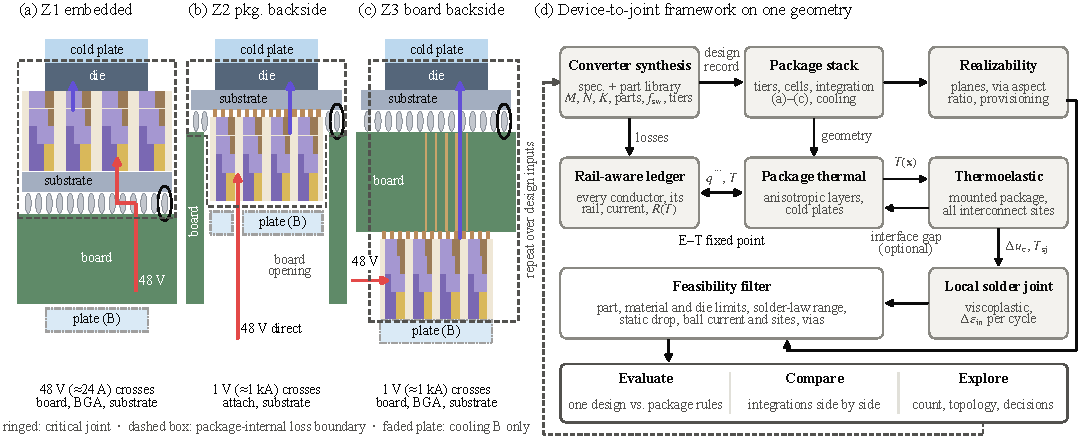
\includegraphics[width=\textwidth]{fig1_concept_framework.pdf}
\caption{(a)--(c) Three integrations of the same regulator cells: embedded between the
substrate and the die (Z1), attached to the substrate backside inside a board opening (Z2), and
mounted on the board backside (Z3). The integration decides which rail crosses the substrate and
the board, at what current, and which solder joints carry the deformation (ringed: critical
joint). The 48-V feed of Z2 and Z3 starts outside the package-internal loss boundary (dashed
box). Schematic; to-scale sections in Fig.~\ref{fig:sections}. (d) The framework: what each
stage hands to the next on one geometry. Double arrow: the bidirectional electrothermal (E--T)
fixed point; single arrows: one-way transfers; dotted: the optional mechanical-to-thermal
feedback through the top thermal interface; dashed: the exploration loop over the design
inputs.}
\label{fig:concept}
\end{figure*}

The framework is a chain of models that share one geometry (Fig.~\ref{fig:concept}). Its inputs
are a system specification---load power and voltage, input rail, die footprint, a target
regulator current density and an allowable ripple---a component library of power devices,
inductors and capacitors, an integration architecture and a cooling solution, given as the
boundaries it imposes (a film coefficient and coolant inlet temperature on each cooled face, or
a coolant model that computes them). Its outputs are a synthesized regulator, an explicit
package stack, a conductor-level loss ledger, converged temperature, deformation and
joint-response fields, a feasibility verdict, and the uncertainty of each output.

\emph{Converter synthesis} enumerates hybrid switched-capacitor--buck topologies and selects
devices, passives and switching frequency for the specified regulator count by exhaustive
search over a discrete library (Section~\ref{sec:dse}). \emph{Stack construction} turns the
selected components into tiers inside each cell footprint, adds the interlayer
redistribution, places the cells in the chosen integration and builds the substrate,
interconnect fields, board, ball field and cooling boundaries around them. The \emph{rail-aware
ledger} assigns to every conductor the rail it carries and that rail's current, and evaluates
its resistance from geometry and temperature. The \emph{package thermal model} receives the
ledger as a heat map deposited where each loss is generated and returns temperatures, which
update every temperature-dependent resistance. The converged field drives a
\emph{thermoelastic package model} of the mounted assembly, which searches every legal
solder-joint site for the largest relative displacement, and a \emph{local viscoplastic
submodel} of the critical joint and its alternatives, which returns their inelastic response per
thermal cycle. The \emph{feasibility} stage checks the result against the ratings of the
selected components and the rules of the package: power-device junction temperature, capacitor,
inductor and package-material limits, the validity range of the solder law, via aspect ratio,
pitch and landing area, and ball and attach provisioning.

\emph{One geometry} has a precise meaning here. Every stage derives its domain from one stack
description: the ledger takes conductor lengths, cross sections and counts from it, and the two
finite-element models discretize it into one mesh. Each ledger term names the layer and the
cell footprints that produce it, and these map to element sets of that mesh; the heat deposited
in them equals the ledger total to $10^{-6}$, and the temperature returned to a term is the mean
over the nodes of the same set. The mechanics reads the converged nodal field on the same mesh,
and the local submodel reads the displacement and temperature of a ball site of the same
lattice the ledger provisions. Three different kinds of interaction follow, and the framework
keeps them apart (Fig.~\ref{fig:concept}d). \emph{Coupled solution}: loss and temperature are
solved together, by fixed-point iteration, because each changes the other at first order.
\emph{One-way transfer}: the converged temperature field loads the mechanics, and the critical
joint's displacement and temperature drive the local submodel; nothing is returned.
\emph{Neglected feedback}: the mechanical state does not update the electrical or thermal model
in production. The thermal strain of a copper conductor, $\alpha_{\mathrm{Cu}}\Delta T\approx
0.15$\,\%, changes its resistance two orders of magnitude less than the 20--35\,\% change of
resistivity inside the fixed point, so the electrical feedback is negligible. The thermal
feedback is not always negligible: when a flat cold plate meets a warped die, the thermal
interface thickens where the die falls away. The framework closes this loop as an option, and
Section~\ref{sec:compare} quantifies it. Contact degradation, delamination, intermetallic
growth and damage are outside the intact-package scope.

\begin{figure}[!t]
\centering
\fbox{\begin{minipage}{0.95\columnwidth}\footnotesize
\textbf{Input:} specification, library, integration, cooling boundaries.\\[2pt]
\textbf{1} \;Synthesize the regulator: exhaustive search over topologies, devices, passives
and $f_{\mathrm{sw}}$ under rating, ripple and area constraints (Section~\ref{sec:dse}).\\
\textbf{2} \;Build the stack and the mesh; check via aspect ratio, pitch, landing and
provisioning (Section~\ref{sec:realizability}).\\
\textbf{3} \;Set the region temperatures $T^{0}$.\\
\textbf{4} \;\textbf{repeat}: ledger $L(T^{k})$; deposit $L$ by region (deposit = ledger total);
solve the thermal field with the cooling boundaries; $T^{k+1}$ = region means;\\
\hspace*{1.2em}\textbf{until} $\max|T^{k+1}-T^{k}| < 0.25$~K and $|\Delta P|/P < 10^{-3}$.\\
\textbf{5} \;Solve the thermoelastic package on the converged field; evaluate $\Delta u$ at
every legal ball site.\\
\textbf{6} \;\emph{Optional}: update the interface thickness from the solved warpage and
return to 4, until the warpage changes by less than 1\,\%.\\
\textbf{7} \;Solve the local submodel at the site of largest $\Delta u$ and at the competing
sites (largest $T_{\mathrm{j}}$, corners, the Pareto set in $\Delta u$ and $T_{\mathrm{j}}$);
report the largest response.\\
\textbf{8} \;Check feasibility: junction, component and material temperatures against their
ratings, joint temperature against the solder law, interconnect rules.\\[2pt]
\textbf{Output:} loss by conductor and component, temperatures, warpage, $\du$,
$\deps$, verdicts, and the uncertainty of each.
\end{minipage}}
\caption{One evaluation of the framework. Steps 1 and 2 are analytical (seconds); step 4 is
the only coupled solution; steps 5 and 7 are one-way transfers.}
\label{fig:algorithm}
\end{figure}

Because every stage reads and writes the same geometry, the framework can be used in three ways
(Fig.~\ref{fig:algorithm}). To \emph{evaluate} a design, the chain is run once and every output
is checked against the ratings and rules of the feasibility stage. To \emph{compare}
integration architectures, the same synthesized regulator is placed in each candidate under the
same cooling boundaries; every output is reported side by side, inside explicitly declared loss
boundaries, and candidates that fail a rating are filtered out before any ranking. To
\emph{explore} the design space, converter synthesis is repeated over regulator count and
topology as an electrical screen, the strongest candidates are carried through the coupled
chain, and every package input without a single defensible value is varied on the production
mesh, so that each ranking is reported together with the decisions that can reverse it.

% ============================================================================ CONVERTER + DSE
\section{Converter Synthesis and Design-Space Exploration}\label{sec:dse}

\subsection{Generalized hybrid regulator family}
The regulator is synthesized from a family rather than fixed in advance. The family is the
two-phase hybrid switched-capacitor--buck converter with $N$ switched-capacitor branches ($N$
high-side switches and $N-1$ flying capacitors) and $K$ inductor branches ($K$ low-side switches),
$K_A$ of them driven in the first phase, and the branch-allocation vector $\mathbf{B}$ with
$\sum_i B_i = N$; the duty ratio is $D = NV_{\mathrm{out}}/V_{\mathrm{in}}$~\cite{Abdelzaher2025ECTC,
Abdelzaher2026EPEPS}. The double series-capacitor buck and the dual-phase multi-inductor hybrid
are members~\cite{DSCH,DPMIH44}. A closed-form continuous-conduction loss model evaluates
conduction in the switches with the inductor ripple, the flying-capacitor equivalent series
resistance and the inductor winding resistance, together with high-side overlap, gate-drive and
output-capacitance switching loss. Against circuit simulation of four published
members---$N/K = 2/2$, $3/2$, $4/4$ and $6/2$ at 48-to-1~V, 30~A and 500~kHz with common
components---the model reproduces total loss to $94.4\pm1.5$\,\% (worst case
92.9\,\%)~\cite{Abdelzaher2025ECTC}, and the extended framework to
$95.3\pm1$\,\%~\cite{Abdelzaher2026EPEPS}. Inductor core loss, alternating-current winding
resistance, dielectric loss and dead-time loss are not in the model; Section~\ref{sec:explore}
bounds them for every compared case and every regulator count.

\subsection{Synthesis}
For a specification---output current and voltage, input voltage, a target current density
$J_{\mathrm{t}}$ and ripple limits---the synthesis enumerates every member with at most 15
components ($2N + 2K - 1 \le 15$, $2\le K\le N$), with $K_A = \lceil K/2\rceil$ and $\mathbf{B}$
the balanced allocation of the branches to the two phases~\cite{Abdelzaher2026EPEPS}. For each
member it searches exhaustively over the library parts that pass the hard constraints---every
combination of high-side device, low-side device, inductor, capacitor and switching frequency on a
50-point logarithmic grid from 43~kHz to 200~MHz, up to the inductor's rated frequency---and
returns the combination of lowest loss at 25\,$^\circ$C. The library holds 90 enhancement-mode GaN
transistors, 11 integrated inductors and 8 capacitors. The hard constraints are the device
voltage rating ($\ge V_{\mathrm{in}}/N$ high side, $\ge V_{\mathrm{out}}$ low side), the 5-V gate
rating and the continuous current rating ($\ge I_{\mathrm{out}}/N$ high side,
$\ge \max(\mathbf{B})I_{\mathrm{out}}/N$ low side); the inductor saturation current
($\ge \max(\mathbf{B})I_{\mathrm{out}}/N$) and rated frequency; the capacitor voltage rating;
the inductor ripple ($|\Delta I| < 0.5\,I_{\mathrm{out}}$) and the output ripple
($\Delta V_{\mathrm{out}} < 0.25\,V_{\mathrm{out}}$ with 50~\textmu F per cell); and the area
budget, which compares the largest tier footprint of the stacked cell,
$\max(NA_{\mathrm{HS}}, KA_{\mathrm{LS}}, KA_{L}, (N-1)A_{C})$, with $I_{\mathrm{out}}/J_{\mathrm{t}}$.
$J_{\mathrm{t}}$ is thus a minimum current density: the selected cell occupies 5.61~mm$^2$ of its
\DseFortyNineBudget-mm$^2$ budget, \DseFortyNineJ~A\,mm$^{-2}$. Temperature, manufacturability
and mechanical response are not constraints of the synthesis; they are evaluated afterward on
the package. One synthesis takes 4.6~s on one core. Device on-resistance is scaled with
temperature by the typical normalized curves of the selected parts, $6.0\times10^{-3}$\,K$^{-1}$
for the high-side EPC2014C and $8.0\times10^{-3}$\,K$^{-1}$ for the low-side EPC2057 over
25--125\,$^\circ$C~\cite{EPC2014C_DS2021,EPC2057_DS2025}, and each device is evaluated at the
in-cell temperature of its own tier.
\emph{Capacitor rule (corrected).} In this family the flying capacitor $C_i$ holds
$(N-i)V_{\mathrm{in}}/N$---32 and 16~V for $C_1$ and $C_2$ of the selected cell---while every
switch blocks $V_{\mathrm{in}}/N$. The published synthesis compared every capacitor with
$V_{\mathrm{in}}/N$, which admitted a 25-V part for the 32-V $C_1$. The rule now requires each
flying capacitor's derated rating (80\,\%) to cover its own stress and its effective capacitance
under bias, temperature and tolerance to hold the switching ripple below 10\,\% of its voltage; the
equivalent series resistance is taken at the switching frequency where the vendor publishes it.
Because the flying capacitors are soft-charged through the inductors, only that resistance enters
the loss. Under the corrected rule the 49-cell synthesis returns the same topology, devices and
frequency with a rated 0603 100-V X7T capacitor, 0.27~\textmu F at 32~V and 7.8~m$\Omega$ at
805~kHz (Table~\ref{tab:spec}), which raises the cell loss by 0.06~W; the published rule is kept
as a reproducible legacy configuration.

\begin{figure}[!t]
\centering
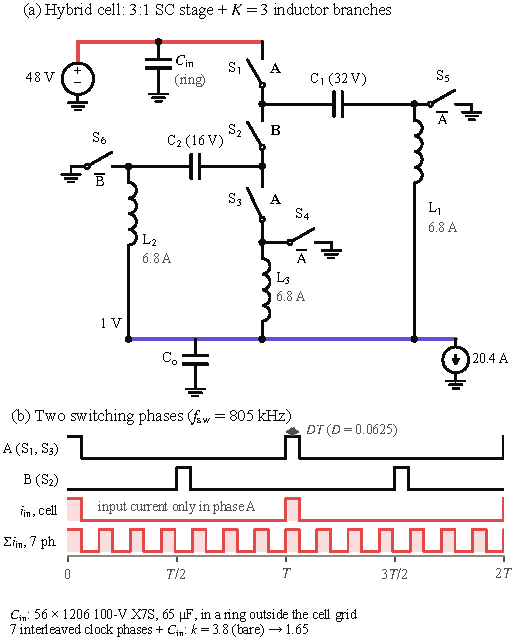
\includegraphics[width=\columnwidth]{fig2_converter.pdf}
\caption{(a) The synthesized cell, $N{=}3$, $K{=}3$, $K_A{=}2$: a 3:1 switched-capacitor stage
(S$_1$--S$_3$; $C_1$ at 32~V, $C_2$ at 16~V) feeding three inductor branches of
$I_{\mathrm{cell}}/3 = 6.8$~A. (b) S$_1$ and S$_3$ conduct in phase A and drive $L_1$ and
$L_3$ at 16~V; S$_2$ conducts in phase B and drives $L_2$; S$_4$--S$_6$ freewheel the undriven
inductors ($D = 0.0625$, $f_{\mathrm{sw}} = 805$~kHz). The 48-V input current flows only in
phase A; $C_{\mathrm{in}}$ is the package input capacitance (56 1206 100-V X7S capacitors,
65~\textmu F at 48~V) in a ring outside the cell grid, and the clocks of the 49 cells are interleaved
in seven phases, which together hold the RMS-to-average ratio of the package input current at
$k = \DecapKeq$ (bare pulse: \DecapKopen; Section~\ref{sec:evaluate}).}
\label{fig:converter}
\end{figure}

\subsection{Regulator count and architecture}
The design-space mode repeats the synthesis over the regulator count $M$ and scores every
candidate with its conversion loss and the system-level routing model of the vertical
interconnect chain and the lateral redistribution path of~\cite{Krishnakumar2026DVPD}, at
25\,$^\circ$C. It is an electrical screen: the strongest candidates are then carried through the
coupled chain (Section~\ref{sec:explore}). Fig.~\ref{fig:dse} shows the screen for a 1-kW,
48-to-1-V load on a 500-mm$^2$ die at $J_{\mathrm{t}} = 3.5$~A\,mm$^{-2}$ over the
\DseNcounts{} counts sampled (\DseCounts). When the topology is re-synthesized at every count,
the selected member changes three times---$N/K = 4/4$, $2/2$, $3/3$ and again $2/2$---and each
jump in Fig.~\ref{fig:dse} is a constraint becoming active: at $M = 40$ the four-branch tier
(7.20~mm$^2$) no longer fits the 7.14-mm$^2$ budget, and at $M = 56$ the smallest three-branch
tier (5.40~mm$^2$) no longer fits 5.10~mm$^2$. Within a member the loss falls with the cell current
and steps when a device, the capacitor or the frequency changes (Table~S2). The minimum lies at
$M = \DseCorrOptM$ ($N2K2K_A1$ at \DseOptFsw~kHz, \DseCorrOptLoss~W under the corrected capacitor rule,
\DseOptLoss~W with the published one), the $3/3$ family reaches its best
at $M = \DseThreeBestM$ (\DseThreeBestLoss~W), and from $M = \DseFirstInfeasibleM$ the budget
(\DseFirstInfeasibleBudget~mm$^2$) is smaller than the smallest two-branch device set that meets
the current rating (3.74~mm$^2$), so no member is feasible. Holding the topology fixed instead
truncates the feasible range at $M = 52$. The seventeen counts take about four minutes on one
core. At $M = 49$ the screen gives \DseFortyNineLoss~W (\DseFortyNineConv~W conversion,
\DseFortyNineRoute~W routing); the package ledger of Section~\ref{sec:models} returns \PIsoZone~W
at 25\,$^\circ$C for the embedded integration---the same conversion loss and a smaller routing
loss from the explicit package conductors---so the two differ only in the routing model.

\begin{figure}[!t]
\centering
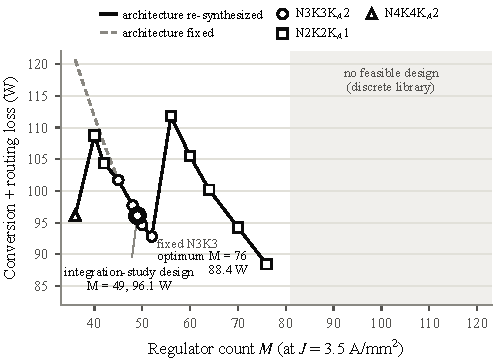
\includegraphics[width=\columnwidth]{fig_dse.pdf}
\caption{(a) Electrical screen of the regulator count: conversion plus system-level routing loss
at 25\,$^\circ$C against $M$ at $J_{\mathrm{t}} = 3.5$~A\,mm$^{-2}$ with the discrete library, topology
re-synthesized at every count under the corrected flying-capacitor rule (solid; markers at the
\DseNcounts{} sampled counts) and the published rule (faded), and held at $N3K3K_A2$ (dashed). Jumps
mark an active area or rating constraint; no member is feasible from $M = \DseFirstInfeasibleM$; the
integration design point is ringed. (b) Package-internal loss of the 49-cell design and of the 64-cell
candidate through the full coupled chain (Z1, cooling~A), a different boundary from the screen.}
\label{fig:dse}
\end{figure}

The integration study of Sections~\ref{sec:evaluate}--\ref{sec:explore} uses one design point
for every architecture, so that any difference between the architectures is caused by the
integration and not by the regulator: $M = 49$ cells on a $7\times7$ grid at
$J_{\mathrm{t}} = 3.5$~A\,mm$^{-2}$, the areal utilization of the reference
framework~\cite{Krishnakumar2026DVPD} and the largest square grid near the electrical screen's
plateau. At that count the search returns the regulator of Table~\ref{tab:spec}---$N3K3K_A2$ with
EPC2014C and EPC2057 devices at 805~kHz, 1.87~W per cell at 25\,$^\circ$C---so the regulator
carried into the package is the synthesis output, not an assumption. Every switch blocks
$V_{\mathrm{in}}/N = 16$~V, 40\,\% and 32\,\% of the high- and low-side ratings; each inductor
carries 6.8~A with 4.7~A of peak-to-peak ripple, a 9.1-A peak against its 23-A saturation current;
the summed cell ripple is 9.0~A (44\,\% of the limit's 50\,\%) and the output ripple 28~mV.

\begin{table}[!t]
\caption{System specification, synthesized design point with ratings and operating stress, and
package and cooling parameters (full material and geometry data: Tables~S1--S4).}
\label{tab:spec}
\centering
\footnotesize
\setlength{\tabcolsep}{2pt}
\begin{tabular}{@{}lL{3.65cm}c@{}}
\toprule
Quantity & Value & Source \\
\midrule
\multicolumn{3}{@{}l}{\emph{Specification (inputs)}}\\
Load / platform rail & 1~kW at 1~V / 48~V & spec. \\
Compute die & $22.36\times22.36$~mm, 1~kW uniform & spec. \\
Regulator count, grid & 49, $7\times7$ & input \\
Target current density $J_{\mathrm{t}}$ & 3.5~A\,mm$^{-2}$, minimum: cell area $\le I_{\mathrm{cell}}/J_{\mathrm{t}}$ & input \\
Ripple limits & $\Delta I < 0.5\,I_{\mathrm{cell}}$; $\Delta V_{\mathrm{out}} < 0.25$~V & input \\
\midrule
\multicolumn{3}{@{}l}{\emph{Synthesized regulator (outputs; rating / operating stress)}}\\
Architecture $N/K/K_A$ & $3/3/2$, $\mathbf{B} = [1,1,1]$, $D = 0.0625$, 805~kHz & synthesis \\
High-side device & EPC2014C: 40~V / 16~V, 10~A, $T_J\le150\,^\circ$C, 16~m$\Omega$ & synthesis \\
Low-side device & EPC2057: 50~V / 16~V, 9.6~A, $T_J\le150\,^\circ$C, 8.5~m$\Omega$ & synthesis \\
Inductor ($\times3$) & 250~nH, 1.6~m$\Omega$, $I_{\mathrm{sat}}$ 23~A / 9.1~A peak, 500~\textmu m, shared-core interposer type~\cite{Rasheedi2026CoupledInductor} & synthesis \\
Flying capacitors $C_1$, $C_2$ & 32~V / 16~V stress. A1: 0603 1~\textmu F 100~V X7T (GRM188D72A105KE01), 0.27/0.59~\textmu F at 32/16~V, 7.8~m$\Omega$, 1.0~mm max; A0: 100-\textmu m tier, no qualifying part & synthesis \\
Output capacitance & 50~\textmu F per cell, in the inductor tier & synthesis \\
Input decoupling & 56 $\times$ 1206 4.7-\textmu F 100-V X7S in a ring outside the grid (65~\textmu F at 48~V); 7 interleaved clock phases; $k = \DecapKeq$ & design \\
Cell footprint & 5.61~mm$^2$ (2.37~mm square), 3.64~A\,mm$^{-2}$ & synthesis \\
Loss per cell at 25\,$^\circ$C & 1.87~W (1.67~W conduction) & synthesis \\
\midrule
\multicolumn{3}{@{}l}{\emph{Package and cooling}}\\
Power substrate & Si, 300~\textmu m, $30\times30$~mm; TSVs 30~\textmu m at 60~\textmu m & \cite{Krishnakumar2026DVPD} \\
Ball-grid array & 0.8~mm pitch, 0.4~mm SAC305 balls & \cite{Krishnakumar2026DVPD} \\
Board & IT-968G, 2.4~mm, homogenized Cu planes & arch. \\
Cold plate (each) & Si microchannels, water at 25\,$^\circ$C, 27~g\,s$^{-1}$, $\Delta p$ \CoolDp~kPa, \CoolPhyd~W hydraulic & design \\
Thermal interface & 50~\textmu m, 3~W\,m$^{-1}$K$^{-1}$ & design \\
\bottomrule
\end{tabular}
\end{table}

% ============================================================================ ARCHITECTURES + MODELS
\section{Integration Architectures and Physical Models}\label{sec:models}

\subsection{Three integrations of one regulator}\label{sec:archs}
The synthesized regulator of Section~\ref{sec:dse} is placed in three integrations
(Fig.~\ref{fig:sections}). All three hold the same \MthNcells{} cells on a
$\MthGrid\times\MthGrid$ grid under the 22.36-mm die, each cell \MthCellSide~mm square at a
\MthCellPitch-mm pitch. They share one converter stack, one tier order and one
\MthBoardMm-mm board, so they differ in placement only (layer stacks: Table~S4).

In the \emph{embedded} integration (Z1), the \MthStackMm-mm converter sits between a
300-\textmu m silicon power substrate and the die. Its 48-V input crosses the board, the 48-V
balls of the BGA, a 48-V RDL on the substrate and the TSVs. Its 1-V output reaches the die through a 10-\textmu m output RDL
and the die pads.

In the \emph{package-backside} integration (Z2), the converter hangs below the substrate inside
a \MthCutout-mm opening in the board, 1~mm from the sidewall. A 30-\textmu m attach of
15-\textmu m Cu pillars at 30-\textmu m pitch joins it to the substrate; thermocompression
bonding at that pitch has been demonstrated on organic substrates~\cite{Au2016CuPillar30um}.
Only the 1-V current crosses the attach and the TSVs. The BGA is a ring of \MthSitesRing{}
sites around the opening, and its power balls carry the 48-V feed. The feed current runs from
the board through these balls and a 48-V RDL on the land side of the substrate to the input pads
of the cells. The lowest face of the converter lies \MthClearZtwo~\textmu m above the underside of
the board.

In the \emph{board-backside} integration (Z3), the converter is attached to the underside of an
uncut board beneath the package, as in current vertical power modules~\cite{Vicor_VPD_AI}. Its
1-V output crosses a board-level solder attach, a field of plated through-holes in the board,
the full BGA and the TSVs. A pair of 48-V copper planes in the board feeds it, and a second cold
plate cools it from below.

\begin{figure*}[!t]
\centering
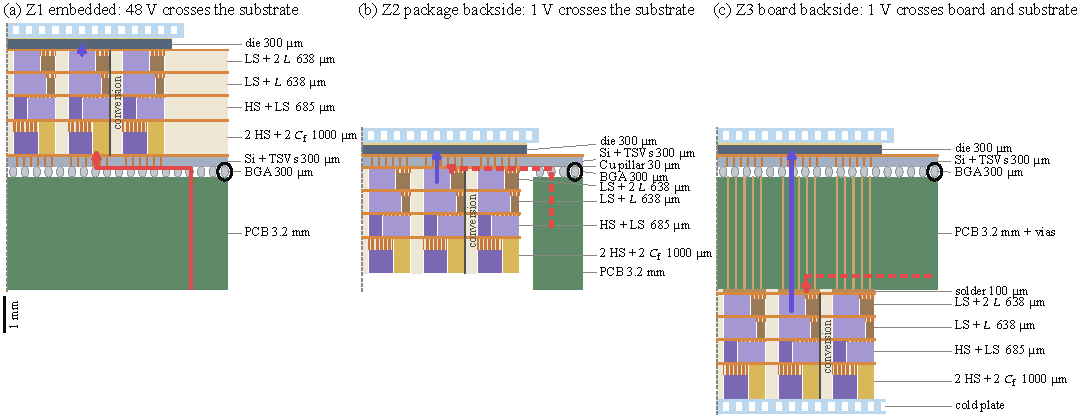
\includegraphics[width=\textwidth]{fig3_sections.pdf}
\caption{The three integrations as meshed: half sections, to scale in $z$ (10-\textmu m RDLs
drawn as lines). Every converter tier holds the parts of its design-record tier; copper posts
(hatched) fill the height above parts shorter than the tier. (a) Z1: converter between
substrate and die, full BGA. (b) Z2: converter in the board opening below the substrate; its
48-V feed runs through the BGA ring and the substrate (dashed). (c) Z3: converter on the board
underside with its own cold plate; the full BGA carries the 1-V output. Red: 48-V path; violet:
1-V path; ringed ball: the outermost row, which holds the critical (corner) joint in every
compared case.}
\label{fig:sections}
\end{figure*}

\subsection{Converter stack, tier order and vertical interconnect}\label{sec:realizability}
The parts of a cell are packed into at most four tiers, and a tier may mix part classes
(Section~\ref{sec:dse}). Each part keeps its body footprint and a \MthKeepout-\textmu m keep-out
in a two-dimensional placement. Listed from the 48-V input end, the first tier holds two
HS dies and both flying capacitors (\MthTierOne~\textmu m). The second holds an HS and an LS die
(\MthTierTwo~\textmu m), the third an LS die and an inductor
(\MthTierThree~\textmu m), and the fourth an LS die and two inductors (\MthTierFour~\textmu m).
With its 10-\textmu m interlayer RDLs, the converter is \MthStackUm~\textmu m tall.

A tier is as tall as its tallest part: the rated 0603 capacitor (\MthHtCf~\textmu m maximum
height), the EPC2014C (\MthHtHs~\textmu m with its terminals) or the EPC2055
(\MthHtLs~\textmu m). Copper posts on the terminals bridge every shorter part to the RDLs above
and below it. They are sized to each die's datasheet land pattern, to the electrode bands of the
capacitor and to the inductor current at 100~A\,mm$^{-2}$. We assume dies with terminals on both
faces, so a die connects through the capture planes on both sides of its tier; single-face
terminals are treated as a sensitivity below.

Whether two parts in different tiers can be connected depends on the conductor planes between
them. An interlayer RDL is patterned copper and serves as a capture plane, so a via must cross
only the dielectric depth of the tiers in between. Each vertical net is checked against the via
count of~\eqref{eq:via}, the pitch, the landing area of the part and the aspect ratio of every
via level. The declared rules are those of chip-embedding
substrates~\cite{Ostmann2008ChipEmbedding}. Laser-drilled \MthViaD-\textmu m microvias cross a
build-up dielectric, every RDL carries a capture pad 1.5 times the via diameter, and each via
level has an aspect ratio of at most 1. This limit is the stacked-microvia practice of
high-density boards~\cite{IPC2226A2017,Ning2019MicroviaFatigue}.

The tier order is chosen in three steps. First, only orders that meet the via rule are kept; if
none does, the orders with the best worst-case aspect ratio are kept. Second, the order of least
intra-cell routing loss is taken. This loss uses the conductor model of the ledger at
25\,$^\circ$C, with the bare input factor on the 48-V nets (Sections~\ref{sec:scenarios}
and~\ref{sec:ledger}). Each order carries the assignment of parts to tiers that routes with the
least loss. Third, orders within \MthRouteTie~W of the least loss are separated by their heat
path, a one-dimensional estimate of the temperature rise from each tier's loss to the die-side
face.

None of the \MthNorders{} orders of the four tiers meets the via rule (Fig.~\ref{fig:realize}).
Every order must cross the \MthTierOne-\textmu m capacitor tier, so its worst via level has an
aspect ratio of \MthWorstAR. That crossing therefore needs copper posts, not build-up vias. The
least routing loss is \MthRouteLeast~W, and \MthNtie{} orders lie within \MthRouteTie~W of it.
Among them the heat path selects the order listed above. It routes \MthRouteChosen~W inside
the cells and has a \MthHeatChosen-K heat path, against \MthHeatLeast~K for the least-loss
order. The same order with its worst part assignment would route \MthRouteWorst~W. Regrouping
the parts into every packable set of at most four tiers (\MthNgroupings{} groupings, \MthNregroup{}
orders) does not remove the posts either: the best worst-case aspect ratio is \MthRegroupAR.

Two sensitivities test this verdict. With a 100-\textmu m capacitor tier the stack shrinks to
\MthThinStackMm~mm, but every order still crosses a device tier, at an aspect ratio of at least
\MthThinAR. With single-face terminals the rule selects the same order, and its worst aspect
ratio stays \MthSingleAR. The verdict is geometric feasibility under declared rules, not a
demonstrated process. Placement within a tier, encapsulation and warpage during lamination are
not evaluated (Section~\ref{sec:discussion}).

The four-tier limit also constrains the converter. The five-tier optimum at the same count
($N4K4$, \MthFswFive~kHz) has a lower electrical loss but a \MthStackFiveMm-mm stack. Hung in the
opening of Z2, it would protrude \MthProtrude~\textmu m below the board
(Section~\ref{sec:explore}).

\begin{figure}[!t]
\centering
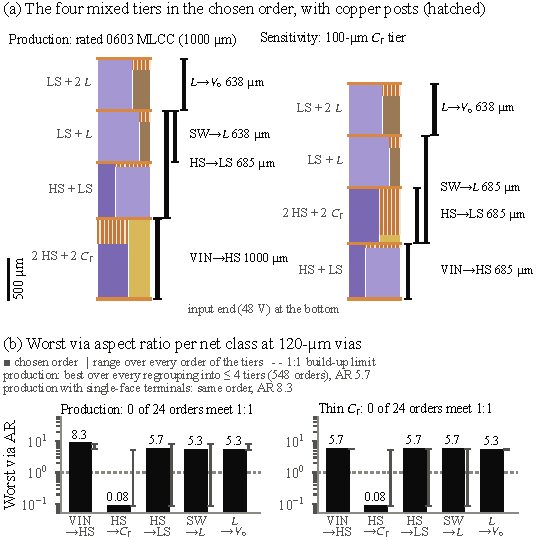
\includegraphics[width=\columnwidth]{fig4_realizability.pdf}
\caption{Tier order as a realizability constraint. (a) The four mixed tiers in the chosen
order, to scale, with the rated 0603 capacitor (production, \MthTierOne-\textmu m tier) and with
a 100-\textmu m capacitor tier (sensitivity); copper posts (hatched) fill the height above
shorter parts, and a bar marks each net class that must cross a whole tier. (b) Worst via
aspect ratio per net class at \MthViaD-\textmu m vias against the 1:1 build-up limit. No order
of either stack meets it, so copper posts make every whole-tier crossing.}
\label{fig:realize}
\end{figure}

\subsection{Input states}\label{sec:scenarios}
The hybrid cell draws input current only in phase $\phi_1$ (Fig.~\ref{fig:converter}b). The RMS
current of the 48-V path therefore depends on how much of that pulse local decoupling absorbs.
We describe it by the RMS factor $k_{\mathrm{rms}}$, the ratio of the RMS to the average 48-V
current. Three input states bound it. \emph{Ideal decoupling} ($k_{\mathrm{rms}} = 1$) is the
limit of unlimited local capacitance. \emph{Bare decoupling} passes the pulse at the buck duty
$D$ unfiltered, $k_{\mathrm{rms}} = 1/\sqrt{D} = \MthKbare$. \emph{Implemented decoupling} is
the production state. Its \MthNphases{} clock phases run in two interleaved groups of six, and a
ring of \MthNring{} 1206 capacitors sits outside the cell grid. Together they give
$k_{\mathrm{rms}} = \MthKeq$ in the package network (Section~\ref{sec:evaluate}). The input
loop inside each cell still carries the bare pulse of the cell, $k_{\mathrm{rms}} = \MthKcell$
from a circuit model of its waveform. Ideal and bare decoupling serve as references.

\subsection{Rail-aware conductor ledger}\label{sec:ledger}
Loss is reported inside a declared boundary. The package-internal loss $P_{\mathrm{int}}$ of Z2
and Z3 starts at the 48-V input terminals of the converter. That of Z1 starts at its 48-V BGA
pads, where the 48-V node of the board, common to all three, meets the package. The board's 48-V
distribution upstream of that node is common to all three and excluded. The external feed of a
backside integration, from that node to the converter, has the loop resistance $R$ and costs
\begin{equation}
P(R) = P_{\mathrm{int}} + \left(k_{\mathrm{rms}} I\right)^2 R,\qquad
V_{\mathrm{in}}\, I = P_{\mathrm{load}} + P(R),
\label{eq:feed}
\end{equation}
where $V_{\mathrm{in}} = 48$~V, $P_{\mathrm{load}} = 1$~kW, $I$ is the average input current and
$k_{\mathrm{rms}}$ the RMS factor of the current the feed carries. Equation~\eqref{eq:feed} is
solved for $I$ by fixed-point iteration. The feed loss is dissipated outside the package and is
not deposited in its thermal model. The same factor scales the package 48-V network of Z1: the
pulsed input current is charged wherever it flows. The crossover $R^{\ast}$ at which a backside
integration loses its advantage over Z1 is a specification for the feed. Two physical feeds are
evaluated against it. The ring feed of Z2 is solved with the same network model as Z1, a
\FeedRbgaZtwo-m$\Omega$ loop. The plane pair of Z3 is two \MthFeedPlaneT-\textmu m copper planes
under the cell grid, a \FeedRZthree-m$\Omega$ loop.

Every conductor carries the rail assigned to it and the RMS current that flows in it. Switched
nets inside the cell carry the RMS currents of the converter model, and the 48-V nets carry
$k_{\mathrm{rms}} I$. The 1-V path carries the RMS cell output current, \MthIoutRatio{} times its
\MthIcell-A average. A vertical field of vias of radius $r$, liner $t_\ell$ and height $h$
carrying the current $I$ is provisioned at a design current density $J_{\mathrm{d}}$ and resolved
by its allocated count,
\begin{equation}
\begin{aligned}
n_{\mathrm{req}} &= \left\lceil \frac{I}{J_{\mathrm{d}}\pi(r-t_\ell)^2}\right\rceil \le
n_{\mathrm{alloc}} \le n_{\mathrm{avail}},\\
R &= \frac{\rho(T)\,h}{\pi(r-t_\ell)^2\,n_{\mathrm{alloc}}},
\end{aligned}
\label{eq:via}
\end{equation}
where $r-t_\ell$ is the copper radius inside the liner, $\rho(T)$ the copper resistivity at the
converged temperature of the field and $n_{\mathrm{avail}}$ the count the pitch rule fits in the
footprint. Inside the cell $J_{\mathrm{d}} = 100$~A\,mm$^{-2}$. Contact and intermetallic
resistances at via and joint interfaces are not resolved; the attach and pad terms carry them
as an all-solder bound. A lateral run is a sheet whose required width must fit the available
width. A link between parts in different tiers is a via stack across the actual tier order, a
link within a tier is a lateral run, and the output plane of the cell is a finite-volume sheet.

Under each cell, \MthTsvCell{} TSVs of 30~\textmu m at 60-\textmu m pitch carry 48~V in Z1 and
1~V in Z2 and Z3. The package 48-V network of Z1 and the ring feed of Z2 are each solved as two
voltage-fed resistive sheets, supply and return. Every ball and pad feeds the sheets through its
own resistance, on a finite-volume grid aligned with every pad and ball edge. The ball currents
are therefore an output. The Cu-pillar attach of Z2 (\MthPillarCell{} pillars per rail and cell)
and the solder attach of Z3 (\MthZthreeBumps{} bumps per rail and cell) are resolved on their
lattices as series columns with two-sided constriction. In Z3, \MthPthCell{} plated
through-holes per rail and cell carry the 1-V current through the board.

The 48-V balls of Z1 and of the ring of Z2 are provisioned by one rule. The current of a ball is
the largest DC ball current of the solved network, scaled by $k_{\mathrm{rms}}$. The count is the smallest
legal (mirror-symmetric) count on the 0.8-mm lattice that holds this current to
\MthBgaTarget~A per ball. This target is a design assumption for 0.4-mm SAC305 (Sn3.0Ag0.5Cu)
balls~\cite{Kuan2015Imax}. A conservative \MthBgaTargetSens-A target is a sensitivity (Section~\ref{sec:explore}).
The power balls may occupy at most \MthLimSites~\% of the sites of the package; the rest carry
signal and auxiliary rails. The harmonic port model of Z1, with every ball tied to an ideal board
node, bounds its worst ball at \MthBgaRmsBound~A RMS. This bound exceeds the target and is
discussed as a limitation (Section~\ref{sec:discussion}).

In Z3 the 1-V current of each rail is shared equally by balls that cover most of the BGA, while
the TSV fields that carry it to the die sit only under the cells. The current of every ball
outside a cell footprint therefore travels laterally, in a land-side copper plane of the
substrate and in the 1-V planes of the board. Each sheet costs
\begin{equation}
\begin{aligned}
P &= \kappa\, R_{\mathrm{s}}(T)\, I_{\mathrm{r}}^2,\qquad
\Delta V = \kappa_V R_{\mathrm{s}}(T)\, I_{\mathrm{r}},\\
R_{\mathrm{s}}(T) &= \rho(T)/(\varphi\, t_{\mathrm{Cu}})
\end{aligned}
\label{eq:sheet}
\end{equation}
for a rail current $I_{\mathrm{r}}$, where $\kappa$ and $\kappa_V$ are shape factors, $t_{\mathrm{Cu}}$
the copper thickness and $\varphi$ its occupancy. The shape factors come from a two-dimensional
finite-volume solution of one rail's sheet. Equal ball currents are its sources, and the TSV or
via fields under the cells are its sinks. Halving its \MthLandGrid-mm grid changes them by
\MthLandGridChk~\%. The land side gives $\kappa = \MthLandKappa$ per rail at
$t_{\mathrm{Cu}} = \MthLandT$~\textmu m and $\varphi = \MthLandOcc$~\%. The board planes are
\MthPlaneN{} declared \MthPlaneT-\textmu m planes per rail at $\varphi = \MthPlaneOcc$~\%, with
$\kappa = \MthPlaneKappa$ for both rails together. Each $R_{\mathrm{s}}$ is evaluated at the
converged temperature of its layer, and the redistribution heat is deposited along its
finite-volume loss map.

\subsection{Package thermal model and cooling}\label{sec:thermal}
Steady conduction $\nabla\!\cdot(\mathbf{k}\nabla T) + q''' = 0$ is solved on the explicit
stack with orthotropic conductivity. Layers that contain regular arrays (TSV fields, attaches,
RDL tiers, ball fields and the board via field of Z3) carry homogenized tensors, each checked
against an explicitly meshed unit cell (Section~\ref{sec:verification}). Every ledger term is
deposited in the layer and cell footprints that produce it. The deposited heat equals the
ledger total to round-off, a relative $\MthDepositResid$.

Each converter tier carries a card homogenized on a unit cell of its contents. Every part is a
vertical column spanning the tier: a series stack of its own layers and, above a shorter part,
its copper posts in encapsulant. The columns and the encapsulant act in parallel through the
thickness; in plane, the midpoint of the series--parallel bracket is used. The posts raise the
through-thickness conductivity of the input-end tier from \MthKzTierOneEncap{} to
\MthKzTierOne~W\,m$^{-1}$K$^{-1}$, and across the four tiers it lies between \MthKzLo{} and
\MthKzHi~W\,m$^{-1}$K$^{-1}$. Sizing the posts to the terminal RMS currents (lower bound) or to
the terminal outlines (upper bound) spans \MthKzPostLo--\MthKzPostHi~W\,m$^{-1}$K$^{-1}$; both
bounds are run as variants (Section~\ref{sec:explore}).

The top boundary is a silicon microchannel cold plate (Table~S5) on a 50-\textmu m thermal
interface material (TIM; 3~W\,m$^{-1}$K$^{-1}$, \TimH~kW\,m$^{-2}$K$^{-1}$). Its effective coefficient
follows from the channel geometry and the flow,
\begin{equation}
\begin{aligned}
h_{\mathrm{eff}}^{-1} &= A_{\mathrm{f}}\left(R_{\mathrm{conv}} + R_{\mathrm{base}}\right),\quad
R_{\mathrm{conv}} = \frac{1}{h_{\mathrm{ch}}\Lambda A_{\mathrm{f}}},\\
\Lambda &= \frac{n L_{\mathrm{ch}}(w + 2\eta_{\mathrm{f}}H)}{A_{\mathrm{f}}},\quad
h_{\mathrm{ch}} = \frac{\mathrm{Nu}\,k_{\mathrm{f}}}{D_{\mathrm{h}}},\\
\eta_{\mathrm{f}} &= \frac{\tanh(mH)}{mH},\quad
m = \left(\frac{2h_{\mathrm{ch}}}{k_{\mathrm{s}}t_{\mathrm{f}}}\right)^{1/2},
\end{aligned}
\label{eq:heff}
\end{equation}
for $n = 223$ channels of width $w = 50$~\textmu m, depth $H = 300$~\textmu m and length
$L_{\mathrm{ch}} = 22.36$~mm over the footprint $A_{\mathrm{f}}$. The fins are silicon
($k_{\mathrm{s}}$) of thickness $t_{\mathrm{f}} = 50$~\textmu m, $D_{\mathrm{h}}$ is the
hydraulic diameter, $k_{\mathrm{f}}$ the water conductivity, and $R_{\mathrm{base}}$ the
resistance of a 100-\textmu m silicon base. A channel is heated on three walls (the base and both fins)
under the H1 condition, with an adiabatic cover. Its fully developed laminar Nusselt number is
$\mathrm{Nu} = \CoolNu$ at aspect ratio 1/6~\cite{ShahLondon1978,QuMudawar2002}. Water enters
at 25\,$^\circ$C at 27~g\,s$^{-1}$ per plate. Its properties are taken at the mean bulk
temperature, \MthTbulk\,$^\circ$C at 1~kW~\cite{NISTWebBook}. The coolant warming
$T_{\mathrm{f}}(x) = T_{\mathrm{in}} + Q(0\!\to\!x)/(\dot m c_p)$ is resolved along every pass
and iterated with the solid solution. The coefficient therefore excludes the caloric resistance
$1/(2\dot m c_p)$ of a uniform sink, which would count half of the coolant rise twice
(Section~\ref{sec:explore}).

A single 22.36-mm pass would need \CoolDpSinglePass~kPa. The plate is therefore a manifold of
\CoolZones{} streamwise zones with alternating inlet and outlet headers, and each pass is
\CoolPassMm~mm long. The flow is laminar ($Re = \CoolRe$) and is taken as uniform over the
channels and zones. With entrance, plenum, turn and header losses of
handbook order~\cite{Idelchik1996}, the pressure drop is \CoolDp~kPa, \CoolDpRatio{} times
below the single pass. The hydraulic power is \CoolPhyd~W per plate, or
\CoolPshaftLo--\CoolPshaftHi~W at the shaft for pump efficiencies of 0.75 to 0.35. The thermal
entry length (\CoolLth~mm) is \MthLthRatio{} of a pass. The fully developed Nusselt number is
thus a lower bound, and the pass-mean coefficient could be up to \MthNuDevRatio{} times higher.

Cooling~A is this top plate alone. Cooling~B adds an identical plate beneath the cell grid,
behind the same TIM. Its flow is sized so that its coolant rises as much as that of the top
plate: \MthBotFlowZtwo~g\,s$^{-1}$ for the \MthBotQZtwo~W that reach it in Z2. Pumping counts
every plate at its own flow. The die dissipates its 1~kW uniformly; a hot-spot map is a
sensitivity (Section~\ref{sec:explore}). The board is a $30\times30$-mm coupon with natural
convection (10~W\,m$^{-2}$K$^{-1}$) beneath it.

The temperature-dependent terms are iterated with the thermal solution to a fixed point: the
on-resistance of each device, the inductor winding and the resistivity of every conductor. Each
term is evaluated at the mean temperature of the region it is deposited in. Each device sits at
the in-cell temperature of its own tier and uses its own datasheet coefficient. The iteration
stops when every coupled temperature changes by less than 0.25~K and the loss by less than
0.1\,\%. It converges in \MthEtItersLo--\MthEtItersHi{} thermal solves and contracts
geometrically. Each loss change is \MthEtContractLo--\MthEtContractHi{} times the previous one;
the largest factor belongs to \MthEtContractCase. The on-resistance coefficients are fitted to
the datasheet curves over 25--125\,$^\circ$C; above that range they are extrapolated, which the
feasibility stage reports.

\subsection{Thermoelastic package and interconnect search}\label{sec:mechanics}
The converged temperature field loads an FE model of the mounted assembly,
$\boldsymbol{\sigma} = \mathbf{C}:(\boldsymbol{\varepsilon}-\boldsymbol{\alpha}(T-T_{\mathrm{ref}}))$
with $T_{\mathrm{ref}} = 25\,^\circ$C. It uses incompatible-mode hexahedra and cubic silicon;
the board and the ball field are meshed as real layers, and only rigid-body motion is
restrained. With this reference the solution is the change from power-off to the operating
point, the excursion that the local cycle imposes. The moduli and coefficients of thermal
expansion (CTE) are those of Table~S3. The encapsulant between the cells and the thickness and
boundary of the board are declared; their alternatives are rerun on the production mesh
(Section~\ref{sec:explore}).

Every interconnect layer is searched rather than assumed: the BGA, the die microbumps, and the
Cu-pillar attach of Z2 or the solder attach of Z3. At every site of a layer of height $h$, the
shear driver is $\gamma = \Delta u/h$, with the relative in-plane displacement across the layer
\begin{equation}
\Delta u = \left\| \mathbf{u}_{\mathrm{t}} - \mathbf{u}_{\mathrm{b}} \right\|_{xy}
\label{eq:du}
\end{equation}
taken from the nodal displacements on its top and bottom planes, interpolated at the site. The
BGA sites are the \MthSitesFull{} legal sites of the 0.8-mm lattice (\MthSitesRing{} in the
ring of Z2); the thinner layers are evaluated at every mesh node. The BGA joint of largest
$\Delta u$, with the displacement $\du$ at its local temperature $T_{\mathrm{sj}}$, drives the
local submodel. The largest displacement need not give the largest inelastic response, so the
submodel is also solved at competing sites (Section~\ref{sec:verification}).

When the optional interface feedback is enabled, the solved warpage sets the local thickness of
the top TIM. The plate is taken as flat and rigid, resting on the highest point of the warped
die at the nominal 50-\textmu m bond line. The TIM thickens by $g(x,y) = \max u_z - u_z(x,y)$,
so the local coefficient becomes $(h_{\mathrm{eff}}^{-1} + g/k_{\mathrm{TIM}})^{-1}$. The fixed
point and the thermoelastic solution are then iterated until the warpage changes by less than
1\,\%. A conforming TIM ($g = 0$, the production chain) and a rigid plate on the free warpage
bound this feedback.

\subsection{Local solder response}\label{sec:local}
The submodel resolves the critical joint, a 400-\textmu m SAC305 ball 300~\textmu m tall at
0.8-mm pitch~\cite{Krishnakumar2026DVPD}. It is meshed as the equal-area 354.5-\textmu m square
prism between two 20-\textmu m copper pads, on four nested hexahedral meshes (L0--L3). The
lower pad face is fixed. The upper face is displaced in plane by $\du$ (its other components
restrained) for a 300-s dwell at $T_{\mathrm{sj}}$ and returned for a 300-s dwell at
25\,$^\circ$C. Every load change is ramped linearly over 3~s and then held. This prescribed cycle stands in
for power cycling between off and the converged operating point; the thermal transient between
them is not modeled.

The solder is elastic--viscoplastic with $E = 45 - 0.12(T-25)$~GPa. Its room-temperature value is
the midpoint of the band of~\cite{Paska2024SAC305}; the slope, $\nu = 0.36$ and the CTE of
21.5~ppm\,K$^{-1}$ are assumed. The production law adds a temperature-dependent yield stress
with isotropic hardening that saturates at 2\,\% inelastic strain~\cite{Yuan2023SAC305}. Creep of
the overstress follows a Norton law,
$\dot\varepsilon_{\mathrm{in}} = A(T)\langle\sigma_{\mathrm{vm}}-\sigma_y\rangle^{n(T)}$, fitted
to tensile creep data~\cite{Xiao2005SAC} (parameters and sources: Tables~S9 and~S10). Those
data cover 45--150\,$^\circ$C and
\MthCalLo--\MthCalHi~MPa, for a Sn3.9Ag0.6Cu alloy rather than SAC305. Between the 5th and
95th percentiles of dwell time, the joints carry \MthVisHotLo--\MthVisHotHi~MPa hot and
\MthVisColdLo--\MthVisColdHi~MPa cold.
The law is therefore extrapolated in stress, and in temperature below 45\,$^\circ$C during the
cold dwell.

Because the production law is extrapolated, the response is carried as a band over two
laws. The second is the Garofalo law of~\cite{Schubert2003ECTC}, entered as a zero-yield Norton
surrogate refitted at each temperature over the stress window the joints visit. The window and
the responses are iterated to self-consistency; after \MthRefitIters{} fits the window settles
at \MthRefitHotLo--\MthRefitHotHi~MPa hot and \MthRefitColdLo--\MthRefitColdHi~MPa cold. Every
joint-response comparison is judged under both laws (Section~\ref{sec:verification}).

The response is the per-cycle increment of accumulated equivalent inelastic strain on the
stabilized (48th) cycle, volume-averaged over the solder core,
\begin{equation}
\deps = \frac{1}{V_{\mathrm{c}}}\int_{V_{\mathrm{c}}}\!
\left[\varepsilon^{\mathrm{eq}}_{\mathrm{in}}(t_k)-\varepsilon^{\mathrm{eq}}_{\mathrm{in}}(t_{k-1})
\right]\mathrm{d}V,
\label{eq:deps}
\end{equation}
where $t_{k-1}$ and $t_k$ bound the last cycle. The core $V_{\mathrm{c}}$ excludes a band of
fixed physical width (59~\textmu m, one sixth of the joint side) along the free edge, where the
bimaterial corner is singular. Fixing the band in physical units keeps the averaging volume
identical at every mesh level, which makes the response mesh-convergent; it is a numerical
device, not a statement about where damage occurs. $\deps$ compares integrations: no damage
law, life relation or allowable is applied.

\subsection{Feasibility limits}\label{sec:feasibility}
The feasibility stage checks every candidate before any ranking, and a candidate that fails a
limit is not ranked. The limits are (every case: Table~S19):
\begin{itemize}
\item the GaN junction temperature, $T_{\mathrm{jn}} \le \MthLimGan\,^\circ$C per device tier:
the in-cell maximum of the tier plus the junction-to-case resistance times the device's own
dissipation;
\item the fit range of the on-resistance coefficients, $T_{\mathrm{jn}} \le \MthLimRonFit\,^\circ$C;
\item the capacitor and inductor tiers, $\le \MthLimMlcc\,^\circ$C;
\item the build-up dielectric and the encapsulant, $\le \MthLimBuildup\,^\circ$C, and the board
laminate, $\le \MthLimBoard\,^\circ$C (glass transitions);
\item the processor die, $\le \MthLimDie\,^\circ$C;
\item the hottest joint of the all-site search, within the $\le\MthLimSolder\,^\circ$C range of
the solder law and below the \MthLimSolidus-$^\circ$C solidus;
\item the static drop of the 1-V path, $\le \MthLimDrop$~mV per rail;
\item the BGA rule above, with at most \MthLimSites~\% of the sites carrying power;
\item a converged operating point.
\end{itemize}
The via rule is reported but is not a filter: no order meets it, so it becomes a requirement for
copper posts.

% ============================================================================ VERIFICATION
\section{Verification, Uncertainty and Cost}\label{sec:verification}

A chain of models has no single accuracy, so it is verified by three kinds of check, each of which
establishes something different (Table~\ref{tab:verif}; every check: Table~S17). Each reduced model
is solved together with a reference on the same problem and the same machine
(Fig.~\ref{fig:verif}). The discretization of each FE model is measured on nested refinement
ladders. Model-form choices that no reference can settle are carried as alternatives through the
whole chain (Section~\ref{sec:explore}).

\begin{table}[!t]
\caption{What Each Check Establishes and What It Does Not}
\label{tab:verif}
\centering
\footnotesize
\setlength{\tabcolsep}{2pt}
\begin{tabular}{@{}L{2.45cm}L{2.85cm}L{3.2cm}@{}}
\toprule
Check & Establishes & Does not establish \\
\midrule
Homogenized cards vs explicit unit cells & The mixing rule for the declared pattern & Contact and
intermetallic resistance; full-package accuracy \\
Package networks vs 2-D FE & The DC conduction model as implemented & High-frequency
power-delivery behavior \\
Thermal unit cells vs commercial and open-source FE & The thermal solver on representative cells
& Material data; the cooling boundary \\
Complete package vs open-source FE, identical and refined meshes & The assembled solver input;
the production-mesh error from above & Model form \\
Cold plate vs conjugate CFD & The Nusselt and fin model at the CFD flow & Manifold flow
distribution and header losses \\
Thermoelastic vs closed form and FE; iterative vs direct solver & Element, restraint and
solver tolerance & Solder fatigue \\
Nested mesh ladder of every compared case & Signed bias and $U_{95}$ of each output and
difference & Model accuracy \\
Local mesh family, cycles, dwell, ramp, averaging band; critical-joint search & Discretization
and stabilization; the site that governs & Constitutive validity (carried as a three-law band) \\
Fixed point and energy balance & Convergence and conservation of the coupled solution &
Completeness of the physics \\
Converter model vs circuit simulation~\cite{Abdelzaher2025ECTC,Abdelzaher2026EPEPS} & The loss
model on other members of the family & Accuracy at the synthesized point \\
\bottomrule
\end{tabular}
\end{table}

\subsection{Reference Checks}
The direct-current conduction stages are checked against a commercial thermal FE solver (Ansys
Electronics Desktop, AEDT) through the exact analogy between $\nabla\!\cdot(k\nabla T) = 0$ and $\nabla\!\cdot(\sigma\nabla V) = 0$.
The single-TSV resistance and the TSV-field and attach homogenizations agree with it within
\ErrHomogMax\,\%. The series rule for the through-thickness conductivity of an RDL tier, in
contrast, overstates it by \ErrRdlKz\,\% because it ignores constriction onto the copper grid, so
the reference tensor replaces the rule in every result. The board via field and the solder attach
of Z3 use the same mixing rules as the verified TSV and pillar cards, without a separate
reference. The voltage-fed networks of the Z1 package and of the Z2 ring feed agree with an
open-source FE solution~\cite{MOOSE} to \ErrPkgRdlZone{} and \MthErrRingNet\,\%. The thermal solver
agrees with commercial and open-source FE solutions of representative unit cells to
\ErrThermMax\,\% of the temperature rise.

The complete Z1 package, solved by the production path and by the MOOSE heat-transfer
module~\cite{MOOSE} on the identical mesh of \MthFpElems{} hexahedra, agrees to
\FullPkgErrZone~K at the peak and over the nodal field. The problem used the converged heat map
of the ideal-decoupling case and a uniform film on the plate face. This check verifies the
assembled solver input and solve; Section~\ref{sec:verif-disc} measures the discretization.

The thermoelastic element reproduces the bimaterial closed form~\cite{Timoshenko1925} to
\ErrMechClosed\,\% and a commercial structural solution to \ErrMechAedt\,\%. The direct
structural solver of this CalculiX build~\cite{CalculiX} fails at \MthSolverFailElems{} elements,
so the production meshes use its iterative solver. On the \MthSolverElems-element base mesh the
two solvers agree to \MthSolverDu\,\% in $\du$ but only to \MthSolverWarp\,\% in die warpage.
This solver term lies outside $U_{95}$; added to both cases of every resolved warpage comparison,
it leaves \MthSolverHold{} of them resolved.

A conjugate computational fluid dynamics (CFD) solution of one channel half-pitch
(\MthCfdCells{} cells, constant water properties) checks the plate model at the single-pass flow.
With the three-wall H1 Nusselt number, the correlation is within \MthCfdErr\,\% of the CFD in mean
base temperature rise and within \MthCfdDpErr\,\% in pressure drop.

\begin{figure}[!t]
\centering
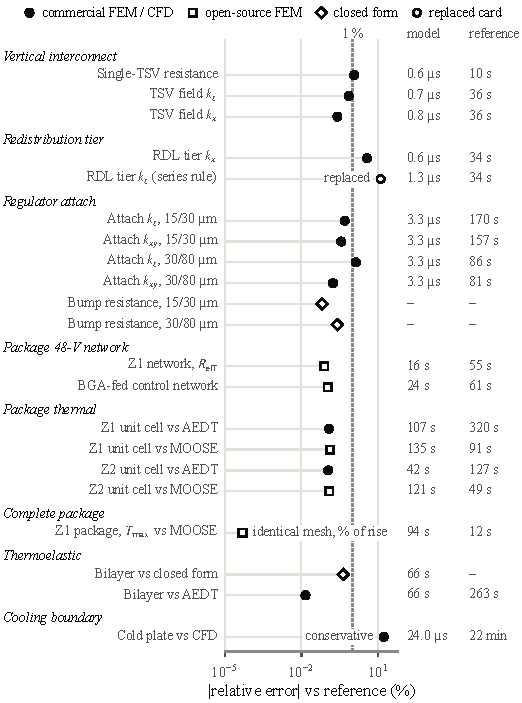
\includegraphics[width=\columnwidth]{fig10_verification.pdf}
\caption{Matched-reference checks: $|$relative error$|$ of each reduced model, and of the
complete Z1 package (CalculiX against MOOSE on the identical mesh), against its reference on the
same problem and machine; right: median runtimes of model and reference. Open marker: the
series-rule RDL conductivity, replaced by the reference tensor in every result; cross: the
iterative against the direct structural solver in die warpage, a term outside $U_{95}$.
Discretization and the local model: Sections~\ref{sec:verif-disc} and~\ref{sec:verif-local}.}
\label{fig:verif}
\end{figure}

\subsection{Discretization and the Resolution Rule}\label{sec:verif-disc}
The package mesh is a graded 1.1-mm grid refined by nested splitting, in which every coarse node
survives; level r$IJ$ splits every in-plane interval into $I$ and every layer into $J$ parts.
Splitting every in-plane interval in two changed the Z1 peak temperature by \MthMeshStepT\,\%, so
the production mesh is r21 (Table~S16). Every compared case, Z1--Z3 under both coolings in the
production state, carries its own ladder of three in-plane levels, r11, r21 and r31. The
ideal-decoupling references of Z1 and Z2 add a through-thickness rung, r12.

MOOSE solutions of the complete Z1 package on uniformly refined copies of up to
\MthFpMaxElems~M hexahedra measure the production-mesh error from above. The die is converged to
\MthFpDie~K. The converter stack, substrate, BGA and board are \MthFpLayerLo--\MthFpLayerHi~K
too cold, converging at an observed order of only \MthFpOrder, and the peak is \MthFpErr~K too
low. The in-plane resolution of the cells causes this error: through-thickness refinement alone
moves the peak by \MthFpTt~K of the \MthFpX~K of a full doubling. For the same case, the bias
plus $U_{95}$ of the production ladder reaches \MthFpBandHi~K and contains this error.

A difference $D = y_b - y_a$ between two cases is \emph{resolved} when $|D+\beta_D| > U_{95}(D)$.
The signed bias $\beta_D$ and the discretization term come from a grid-convergence-index (GCI)
estimate on $D$'s own rung sequence~\cite{Roache1998,Celik2008}. Errors that the two cases share
on one mesh family thus cancel only where they move together. A monotone ladder whose observed
order lies within 0.2 of the formal order 2 is asymptotic and uses the safety factor
$F_s = 1.25$. Other monotone ladders use $F_s = 3$ with the order limited to [0.5,~2]. An
oscillatory ladder carries $F_s$ = 3 times half its range and no signed bias. The bias is
$\beta = e_{32}r^p/(r^p-1)$, with $e_{32}$ the r21-to-r31 change, $p$ the order and $r = 1.5$.

$U_{95}(D)$ adds three terms in quadrature to the discretization term: the through-thickness
split where an r12 rung exists, the fixed-point stop of each case (0.1\,\% of the loss,
0.25~K) and the matched-reference agreement of the solver (0.13\,\% of a temperature
difference, 0.43\,\% of a displacement difference). The coverage is about 95\,\%. Model-form
uncertainty is not part of $U_{95}$. Section~\ref{sec:explore} evaluates both integrations under
each declared alternative, and a resolved ranking that an alternative reverses is conditional on
it.

Of the \MthNcomp{} compared differences in loss, peak temperature, warpage and $\du$
(Table~\ref{tab:uncertainty}; per-case values: Table~S18), \MthNasymWord{} have asymptotic ladders,
\MthNnotasym{} monotone but not asymptotic ones and \MthNoscWord{} oscillatory ones. The rule resolves
\MthNresolved{} of them; only the loss of Z3 against Z1 under cooling~B is not resolved. The
production mesh underestimates every loss, by \MthBiasPLo--\MthBiasPHi~W, and every peak
temperature, by \MthBiasTLo--\MthBiasTHi~K. Testing each difference on its own ladder matters:
under cooling~A, the \GapAZtwo-W loss gap between Z1 and Z2 has $U_{95}(D) =
\WrResAZoneZtwoPlossUni$~W, whereas the two cases' own $U_{95}$ sum to \MthGapAPlossSum~W.

The through-thickness term is measured on the ideal-decoupling references. It moves loss and
peak temperature by at most \MthTtTZone\,\%, but the die warpage of Z1 by \MthTtWarpZone\,\% and
its $\du$ by \MthTtDuZone\,\%. The production ladders lack this rung. Adding the relative term of
the references to every compared case, together with the solver term to every warpage, leaves
\MthTtHold{} resolved differences resolved; the die warpage of Z3 against Z1 under cooling~B is the
exception.

The coupled solution conserves energy. Heat deposited in the mesh equals the ledger total to
round-off (a relative $\MthDepositResid$), and heat leaving through the plate and board films
equals the deposited heat to a relative $\MthEnergyResid$ in every compared case.

\subsection{Local Response and Critical Joint}\label{sec:verif-local}
The local model is verified at the critical joints of the production state (Tables~S12--S14).
Refining its mesh from L0 to L3 changes the six responses by at most \MvMeshUmax\,\%, and eight
cycles leave the four-cycle responses unchanged at the printed precision, so their numerical
$U_{95}$ is at most \MvMeshUmax\,\%. A 60-s or 900-s dwell changes the responses by
\MvDwellSixtyLo{} to \MvDwellNineHundredHi\,\%, and a 30-s ramp by at most \MvRampThirtyHi\,\%;
neither changes a ranking. The averaging core excludes a corner band of
\MthBandProdUm~\textmu m; bands of \MthBandUm~\textmu m, at L0 and L2, change the responses by
\MthBandLo{} to \MthBandHi\,\% and no ordering. The two band laws give
\MvRatioXiaoLo--\MvRatioXiaoHi{} and \MvRatioMeasLo--\MvRatioMeasHi{} times the response of the
production law, and under each law the critical joint is the same site.

The critical-joint search terminated in every case with no unsolved site bounded above the
largest response (Table~S13). Of the \MvCritLattice{} lattice sites of the six cases, it solved
\MvCritSchubSolved{} under the production law and \MvCritSolvedAll{} under the three laws. The
screening features are needed because the response is not monotone in the in-plane displacement
and the joint temperature. In \num[group-separator={,}]{\MvCritViol} of \MvCritPairs{} pairs of
sites ordered by $(\Delta u, T_{\mathrm{sj}})$, the dominated site responds more, by up to
\MvCritViolMax\,\%. In the screening features only \MvCritViolF{} of \MvCritPairsF{} ordered
pairs reverse by more than 1\,\%, by at most \MvCritRevF\,\%, which sets the margin at
\MvCritMarginMin--\MvCritMargin\,\%.

The joint of largest $\Delta u$, or its mirror image within the 1-\% noise of the local model, is
the critical joint in every case except those of Z2. Under cooling~A, the critical joint of Z2 is
an inner site of the ring that responds \MvCritRatioMax\,\% more than the joint of largest
$\Delta u$. Under cooling~B, it is the mirror corner, which responds \MvCritRatioBZtwo{} times as
much because the streamwise coolant breaks the symmetry.

% GENERATED by scripts/tcpmt_uncertainty.py -- do not edit
\begin{table}[!t]
\caption{Numerical uncertainty $U$ of each compared output (S0, production mesh) and the comparisons it resolves: a gap is resolved when it exceeds $2(U_a+U_b)$.}
\label{tab:uncertainty}
\centering
\footnotesize
\setlength{\tabcolsep}{2.5pt}
\begin{tabular}{@{}lrrrrrr@{}}
\toprule
 & \multicolumn{3}{c}{Cooling A: $\pm U$} & \multicolumn{3}{c}{Cooling B: $\pm U$}\\
\cmidrule(lr){2-4}\cmidrule(l){5-7}
Output & Z1 & Z2 & Z3 & Z1 & Z2 & Z3 \\
\midrule
Loss (W) & 0.67 & 0.62 & 0.78 & 0.67 & 0.48 & 0.49 \\
Peak temp.\ (K) & 1.36 & 0.97 & 1.22 & 1.30 & 0.55 & 0.44 \\
Die warpage (\textmu m) & 0.62 & 0.69 & 3.08 & 0.14 & 0.18 & 0.37 \\
$\du$ (\textmu m) & 0.04 & 0.06 & 0.18 & 0.01 & 0.04 & 0.06 \\
$\deps$ ($10^{-3}$/cycle) & 0.19 & 0.25 & 1.63 & 0.04 & 0.03 & 0.30 \\
\midrule
\multicolumn{7}{@{}l}{\emph{Comparisons (lower first; R: resolved, --: within $2U$)}}\\
\multicolumn{7}{@{}p{0.95\columnwidth}@{}}{A, Z1/Z2: Loss Z1 R; Peak temp.\ Z1 R; Die warpage Z1 R; $\du$ Z1 R; $\deps$ Z1 R}\\
\multicolumn{7}{@{}p{0.95\columnwidth}@{}}{A, Z1/Z3: Loss Z1 R; Peak temp.\ Z1 R; Die warpage Z1 R; $\du$ Z1 R; $\deps$ Z1 R}\\
\multicolumn{7}{@{}p{0.95\columnwidth}@{}}{B, Z2/Z1: Loss Z2 R; Peak temp.\ Z2 R; Die warpage Z1 R; $\du$ Z1 R; $\deps$ Z1 R}\\
\multicolumn{7}{@{}p{0.95\columnwidth}@{}}{B, Z3/Z1: Loss Z3 R; Peak temp.\ Z3 R; Die warpage Z1 R; $\du$ Z1 R; $\deps$ Z1 --}\\
\multicolumn{7}{@{}p{0.95\columnwidth}@{}}{B, Z2/Z3: Loss Z2 R; Peak temp.\ Z2 --; Die warpage Z3 R; $\du$ Z3 R; $\deps$ Z3 R}\\
\bottomrule
\end{tabular}
\end{table}


\subsection{Cost}
The analytical stages cost microseconds to minutes. A homogenized card takes microseconds
(Fig.~\ref{fig:verif}), the converter cards of a design \MthCardsSec~s, the tier-order search
\MthTierOrderMin~min and the \FrDseNcounts-count electrical screen \MthDseMin~min. One coupled
evaluation on the production mesh, without the local model, takes \MthTotHLo--\MthTotHHi~h on a two-socket
workstation (Intel Xeon Gold 6342; CalculiX~2.23). The electrothermal fixed point takes
\MthEtMinLo--\MthEtMinHi~min for \MthEtItersLo--\MthEtItersHi{} thermal solves on two threads.
The structural solve with the all-site search takes \MthMechMinLo--\MthMechMinHi~min on one
thread, and geometry and meshing take under 2~min. The critical-joint search adds
\MvCritSolvedAll{} independent solves of the local model over the six cases and three laws; they
parallelize over the sites. The per-stage breakdown, mesh sizes, degrees of freedom and peak
memory are in Table~S16. On the identical package mesh the open-source solver is faster (\FullPkgMooseZone~s
against \FullPkgCcxZone~s on eight cores), because the production path factors the system with a
single-threaded direct solver.

% ============================================================================ EVALUATE
\section{Evaluating a Design}\label{sec:evaluate}

The evaluated design is the embedded regulator (Z1), the integration of the reference
framework~\cite{Krishnakumar2026DVPD}, at the design point of Table~\ref{tab:spec}. It runs in the
production state, with the implemented input decoupling, under cooling~A.
Fig.~\ref{fig:fields}(a), (d) and~(g) show its fields, and the first column of
Table~\ref{tab:compare} gives its numbers.

\subsection{Electrothermal State}\label{sec:evaluate-et}
The fixed point converges in \WrEtItersAZoneWord{} iterations to \PlossAZone~W inside the package, a
package-internal efficiency of \WrEffAZone\,\%. Conversion accounts for \PconvAZone~W, and the
low-side devices alone dissipate \WrPconvLsAZone~W of it (\WrLsShareAZone\,\%). Routing accounts for
\ProuteAZone~W: \WrPintraAZone~W in the cells' own conductors, \WrPhvAZone~W in the package 48-V
network and \WrPringAZone~W in the input capacitors.

The peak, \TmaxAZone\,$^\circ$C, lies in the input-end tier, which holds two high-side devices and
the two flying capacitors. That tier sits farthest from the cold plate: its heat crosses the other
three tiers and the die. The other three tiers peak at \WrTtierTwoAZone, \WrTtierThreeAZone{} and
\WrTtierFourAZone\,$^\circ$C, falling toward the die. The die averages \WrTdieMeanAZone\,$^\circ$C and
peaks at \TdiemaxAZone\,$^\circ$C under its uniform load.

Evaluated with every region at 25\,$^\circ$C, the same ledger returns \WrIsoLoZone~W. An electrical
analysis decoupled from the thermal solution would therefore understate the package loss by
\WrUnderAZone\,\% (\WrRiseAZone~W). The difference is the on-resistance and copper resistivity of
parts that run \WrTlsRiseAZone{} to \WrThsRiseAZone~K above room temperature.

\subsection{Input Decoupling}\label{sec:evaluate-decap}
Capacitance inside the stack does not lower the RMS factor $k_{\mathrm{rms}}$ enough, and neither
does interleaving or a ring alone, so the implemented decoupling (Section~\ref{sec:scenarios})
combines the last two. With the cells in phase and no input capacitance, a port model of the package network
gives $k_{\mathrm{rms}} = \WrKsync$.

Charge balance asks for only \WrCchargeOneV~\textmu F per cell for 1~V of input ripple. A circuit
model of the package loop says otherwise. It includes the loop's inductance, \WrLloop~pH nominal
within \WrLloopLo--\WrLloopHi~pH, and the capacitors' series resistance, series inductance and bias
derating. In that model $k_{\mathrm{rms}}$ falls slowly with capacitance: $k_{\mathrm{rms}} \le 1.2$
needs about \WrCkTwelve~\textmu F per cell at 100~pH.

The embedded stack has no room for that. The gaps between cells hold \WrGapCapsPerCell{} capacitors
per cell, 0402 100-V X7R parts, the largest such part rated to 125\,$^\circ$C. Their few nanofarads
resonate with the package inductance and raise $k_{\mathrm{rms}}$ to \WrKgap{}, and to \WrKgapHi{} at
the worst inductance of the band. A ring of \FrDecapN{} capacitors outside the cell grid, 1206 100-V
X7S parts, holds \FrDecapCtot~\textmu F at 48~V and 105\,$^\circ$C. On its own it gives
$k_{\mathrm{rms}} = \WrKring$, because the package inductance separates it from the cells.
Interleaving the cells' clocks on its own gives \WrKinter.

In the implemented decoupling, \FrDecapPhases{} clock phases form two interleaved
\FrDecapGroupWord-phase groups on a checkerboard, the second offset by half a phase step. With the ring
they reach $k_{\mathrm{rms}} = \WrKrms$, and \WrKrmsLo--\WrKrmsHi{} over the inductance band. An ideal
\FrDseOptM-phase spread with the ring would reach only \WrKspread: the sheet next to each cell still
carries that cell's own pulse.

The implemented decoupling costs \WrDecapCoupledA~W against ideal decoupling in the coupled case.
Of this, \WrHotLoop~W is dissipated in the cells' own input loops, which carry the bare pulse
whatever sits outside the cell. Bare decoupling would cost \RiseSoneZone~W more than ideal
decoupling. It would also put \WrBgaBareAtNmaxZone~A on each 48-V ball even at the legal maximum of
\WrBgaNmax{} balls per rail, beyond the per-ball target. The interleaving is therefore a requirement
on the converter's control, not an option.

\subsection{Package Interface}\label{sec:evaluate-bga}
At the implemented waveform the ball rule of Section~\ref{sec:ledger} gives the 48-V field of Z1
\WrBgaNZone{} balls per rail, the smallest legal count, each carrying \WrBgaIZone~A, on \WrBgaFracZone\,\% of the
\MthSitesFull{} sites. The static 1-V drop from the converter output to the die is
\VdropAZone~mV per rail, within the \MthLimDrop-mV limit.

\subsection{Mechanical State}\label{sec:evaluate-mech}
The die warps by \WarpAZone~\textmu m peak to valley. The largest relative displacement across the
ball layer lies at a corner of the array, $\du = \DuAZone$~\textmu m. The critical joint is that
corner or its mirror image, at $T_{\mathrm{sj}} = \MvTsjAZone\,^\circ$C. It accumulates
$\deps = \MvEpsAZone\times10^{-3}$ per cycle under the production law, with a numerical uncertainty
of \MvEpsUrelAZone\,\%, and \MvEpsLoAZone$\times10^{-3}$ under the lowest law of the band.

Of the other interconnect layers, the \WrHIfUm-\textmu m die-to-converter microbumps carry the
largest driver: $\gamma = \WrGamIfAZone\times10^{-3}$ at \WrTIfAZone\,$^\circ$C, about
\WrGamRatioAZoneWord{} times that of the ball of largest $\Delta u$ ($\WrGamBgaAZone\times10^{-3}$).
Section~\ref{sec:compare-joints} explains why these layers are screened rather than ranked.

\subsection{Feasibility}\label{sec:evaluate-feas}
The evaluated design passes every check of the feasibility stage (Table~S19). The GaN junctions
reach $T_{\mathrm{jn}} = \TjAZone\,^\circ$C, \WrGanMarginAZone~K below their \MthLimGan-$^\circ$C
rating. Three limits bind more tightly than that rating. The hotter junction lies
\WrRonMarginAZone~K below \MthLimRonFit\,$^\circ$C, the upper end of the on-resistance fit, beyond
which the loss model would extrapolate. The flying-capacitor tier peaks \WrMlccMarginAZone~K below
its \MthLimMlcc-$^\circ$C class. The hottest joint lies \WrSolderMarginAZone~K inside the range of the
solder laws. Under its uniform load the die peaks \WrDieMarginAZone~K below its
\MthLimDie-$^\circ$C limit. Section~\ref{sec:explore} shows which explored decisions consume these
margins.

\begin{figure*}[!t]
\centering
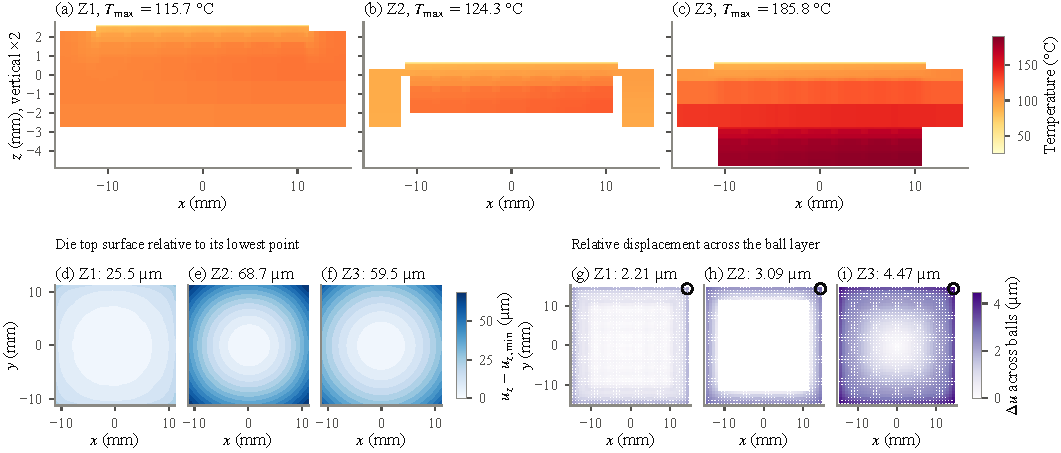
\includegraphics[width=\textwidth]{fig7_fields.pdf}
\caption{Converged fields of the three integrations in the production state (implemented input
decoupling) under cooling~A (one top cold plate). (a)--(c) Temperature on the vertical section
through the middle row of cells (vertical scale doubled; voids left empty; dashed: the
\MthLimGan-$^\circ$C GaN-rating isotherm). (d)--(f) Out-of-plane displacement of the die top surface
relative to its lowest point; its peak-to-valley value is the die warpage. (g)--(i) Relative
in-plane displacement across the ball layer at every legal site. Ring: the joint of largest
$\Delta u$, whose value heads the panel; cross: the critical joint where it is neither that joint
nor its mirror image. Z3 includes its coupled land-side and board-plane redistribution.}
\label{fig:fields}
\end{figure*}

% ============================================================================ COMPARE
\section{Comparing Integrations}\label{sec:compare}

In comparison mode the same synthesized regulator---cell count, topology, devices, passives and
tier stack---is placed in each integration, and every output is reported inside declared loss
boundaries. Because the integrations differ in how the converter can be cooled, they are compared
three ways (Table~\ref{tab:compare}, Fig.~\ref{fig:tiers}): at one common temperature, which is
what an analysis without electrothermal coupling sees; with the same top cold plate (cooling~A);
and with the same top plate and an identical bottom plate under the cell grid, behind the same
50-\textmu m thermal interface as the top plate (cooling~B). Model-form errors common to all
columns---the converter loss model, the device temperature coefficients, the solder
law---largely cancel in the differences.

% GENERATED by scripts/tcpmt_manuscript_macros.py -- do not edit
\begin{table*}[!t]
\caption{The three integrations at S0 under cooling~A (one top cold plate) and cooling~B (top and bottom plates), reference capacitor case A0. Loss inside the package-internal boundary unless stated; $\pm U$: numerical uncertainty (Table~\ref{tab:uncertainty}).}
\label{tab:compare}
\centering
\footnotesize
\setlength{\tabcolsep}{3.5pt}
\begin{tabular}{@{}lrrrrrr@{}}
\toprule
 & \multicolumn{3}{c}{Cooling A: top plate} & \multicolumn{3}{c}{Cooling B: top and bottom plates}\\
\cmidrule(lr){2-4}\cmidrule(l){5-7}
 & Z1 & Z2 & Z3 & Z1 & Z2 & Z3 \\
\midrule
\multicolumn{7}{@{}l}{\emph{Performance}}\\
Loss (W) & 144.3$\pm$1.7 & 147.4$\pm$1.5 & 199.6$\pm$2.0 & 142.6$\pm$1.6 & 115.2$\pm$1.2 & 124.5$\pm$1.2 \\
\quad conversion / routing & 140.7 / 3.6 & 144.8 / 2.7 & 181.4 / 18.1 & 139.1 / 3.6 & 112.9 / 2.3 & 109.7 / 14.8 \\
Peak temperature ($^\circ$C) & 115.7 & 124.3 & 185.8 & 111.3 & 81.5 & 83.3 \\
GaN junction, bound ($^\circ$C) & 116.2 & 124.8 & 186.3 & 112.3 & 67.6 & 61.0 \\
Board, mean ($^\circ$C) & 111 & 93 & 131 & 67 & 75 & 72 \\
Die warpage (\textmu m) & 25.5$\pm$1.5 & 68.7$\pm$1.1 & 59.5$\pm$9.5 & 5.9$\pm$0.3 & 17.6$\pm$0.3 & 7.1$\pm$1.1 \\
$\du$ (\textmu m) at $T_{\mathrm{j}}$ ($^\circ$C) & 2.21 (115.0) & 3.09 (97.2) & 4.47 (109.9) & 0.69 (108.3) & 2.10 (78.7) & 1.56 (80.4) \\
$\deps$ ($10^{-3}$/cycle)\textsuperscript{a} & 5.73$\pm$0.17 & 8.02$\pm$0.08 & 13.48$\pm$0.27 & 1.89$\pm$0.14 & 4.04$\pm$0.13 & 2.32$\pm$0.12 \\
Heat to top / bottom plate (W) & 1144 / 0 & 1147 / 0 & 1198 / 0 & 1130 / 13 & 925 / 190 & 960 / 164 \\
\midrule
\multicolumn{7}{@{}l}{\emph{Loss accounting and platform}}\\
Static 1-V drop to the die (mV)\textsuperscript{b} & 0.04 & 0.83 & 16.0 & 0.04 & 0.78 & 13.3 \\
Feed limit $R^*$ (m$\Omega$) & n/a & none & none & n/a & 48.4 & 32.1 \\
Physical feed loss (W) & -- & 1.17 & 0.12 & -- & 1.10 & 0.10 \\
Pumping, shaft (W) & 31 & 31 & 31 & 61 & 61 & 61 \\
Platform-inclusive loss (W) & 174.9 & 179.2 & 230.2 & 203.8 & 177.4 & 185.7 \\
\midrule
\multicolumn{7}{@{}l}{\emph{Feasibility}}\\
All component and material limits & pass & pass & \textbf{fail} & pass & pass & pass \\
Joint within solder law ($\le125\,^\circ$C) & pass & pass & pass & pass & pass & pass \\
BGA sites carrying power (of 1369) & 108 & 0 & 1334\textsuperscript{c} & 108 & 0 & 1334\textsuperscript{c} \\
Worst via aspect ratio, A0 / A1 & 0.83 / 8.6 & 0.83 / 8.6 & 0.83 / 8.6 & 0.83 / 8.6 & 0.83 / 8.6 & 0.83 / 8.6 \\
Fits the 2.4-mm board opening, A1 & n/a & \textbf{no} & n/a & n/a & \textbf{no} & n/a \\
\bottomrule
\end{tabular}
\par\smallskip\raggedright\footnotesize \textsuperscript{a}Stabilized cycle, L0 mesh. \textsuperscript{b}1-V conductor loss divided by the load current. \textsuperscript{c}Leaves 35 sites for every signal and auxiliary rail: a feasibility failure of this package.  A1: rated MLCC flying capacitors (1030-\textmu m tier).
\end{table*}


\subsection{Placement alone}\label{sec:compare-elec}
At a common temperature the conversion loss is identical by construction, and the integrations
differ only in routing (Fig.~\ref{fig:loss}). Moving the regulator out of the package removes
the package 48-V network, \PhvZone~W in Z1, and sends the kiloampere 1-V current through new
conductors: the Cu-pillar attach and the TSV field in Z2 (\PattZtwo{} and \PtsvZtwo~W), and the
board-level attach, the board via field with the ball field, and the TSVs in Z3 (\PattZthree,
\PboardZthree{} and \PtsvZthree~W). At 100\,$^\circ$C, Z2 is \GapIsoHotZtwo~W below Z1 and Z3
\GapIsoHotZthree~W above it. Z3 pays more than its ledger shows. At 1.5~A per ball its 1-V
current needs 1334 of the 1369 sites of the 0.8-mm ball array, leaving 35 for every signal and
auxiliary rail, and only \LandBallsInside{} balls per rail lie under the cells. The current of
the rest must spread laterally in the land side of the package; a sheet solution of that
redistribution, which the coupled ledger does not contain, adds \LandPmin--\LandPmax~W and
\LandDVmin--\LandDVmax~mV of drop for \LandTmax--\LandTmin~\textmu m of land-side copper.
Carrying the current straight down under the cells would require a ball pitch of
\PitchMaxZthree~mm.

\begin{figure}[!t]
\centering
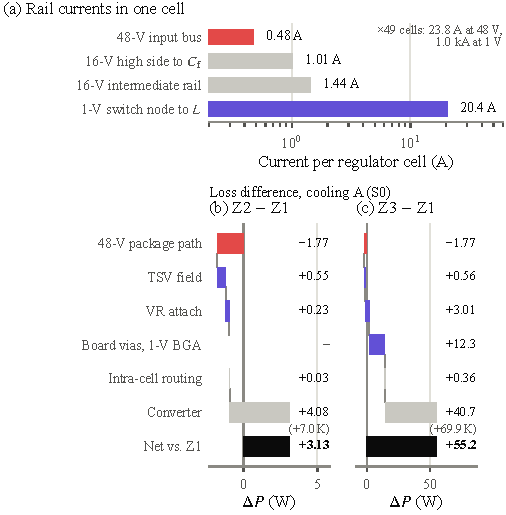
\includegraphics[width=\columnwidth]{fig5_loss_swap.pdf}
\caption{(a) Current per regulator cell in each class of connection, by rail. (b), (c)
Package-internal loss of Z2 and of Z3 minus that of Z1 under cooling~A, term by term: the routing
each integration removes or adds, and the change of conversion loss caused by the converter's own
temperature (low-side tier temperature difference in parentheses).}
\label{fig:loss}
\end{figure}

\subsection{The same top cold plate}
With one top plate the converter's thermal path decides the ranking, and it reverses the
placement-alone result twice. The converter of Z2 is cooled only through the attach and the
substrate, so its low-side tier runs \dTlsAbsZtwoSzero~K hotter than in Z1 and its conversion loss
rises by \dPconvAbsZtwoSzero~W, about \ConvToRouteZtwo{} times the \dProuteAbsZtwoSzero~W it saves
in routing: Z1 has the lower loss, by \GapAZtwo~W. The converter of Z3 must push its heat up
through 2.4~mm of board: it reaches \TmaxAZthree\,$^\circ$C and dissipates \PlossAZthree~W,
\GapAZthree~W more than Z1. The cooling solution of the embedded and package-backside
integrations does not survive the board-backside one. Mechanically, Z1 sandwiches the converter
between the die and the substrate on the full ball array and its die warps by \WarpAZone~\textmu m;
Z2 is a thin silicon plate that carries the encapsulated converter on one side and rests on a
ring of balls around the opening, a bimetal strip whose die warps \WarpRatioZtwo{} times as much
and whose critical joint moves \DuRatioZtwo{} times as far (Fig.~\ref{fig:fields}).
% TODO(data): Z3 under cooling A, mechanical sentence

\begin{figure*}[!t]
\centering
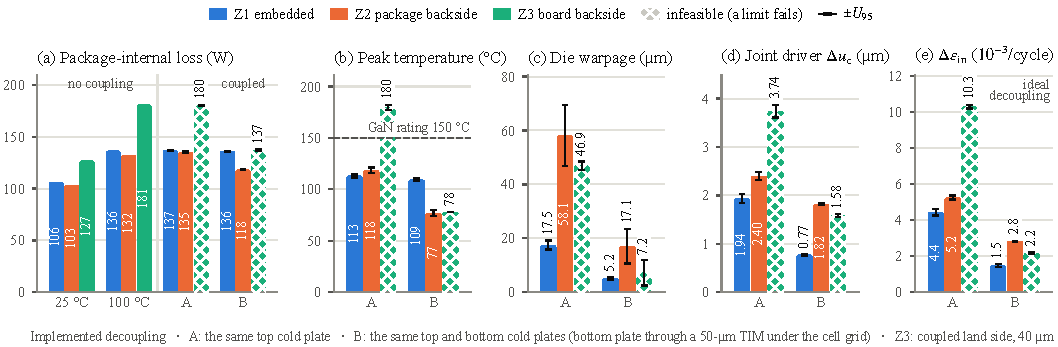
\includegraphics[width=\textwidth]{fig8_tiers.pdf}
\caption{The three integrations at S0 compared three ways. (a) Package-internal loss at one
common temperature (no electrothermal coupling) and coupled under cooling~A (the same top cold
plate) and cooling~B (the same top and bottom plates). (b) Peak temperature, (c) die warpage and
(d) critical-joint displacement under cooling~A and~B. Open diamonds: the interface-free bottom
plate, a bound.}
\label{fig:tiers}
\end{figure*}

\subsection{The same top and bottom cold plates}
% TODO(data): cooling B results -- which integration can use the bottom plate (Z1 only through
% substrate, balls and 2.4 mm of board; Z2 and Z3 directly), losses, temperatures, warpage, joints;
% the interface-free bound; R* under B.

The direct 48-V feed of the backside integrations lies outside the package boundary; its loop
resistance enters through~\eqref{eq:feed} and is treated as a requirement (Fig.~\ref{fig:feed}).
Where a backside regulator is ahead at zero feed resistance, $R^*$ is the largest loop resistance
that keeps it ahead; where it is behind, no feed recovers the difference. Under cooling~A, Z2 is
behind at S0 and needs a loop below \RstarZtwoSone~m$\Omega$ at S1, about \RstarOverLoopZtwo{}
times the package 48-V loop of Z1 (\RloopZone~m$\Omega$).

\begin{figure}[!t]
\centering
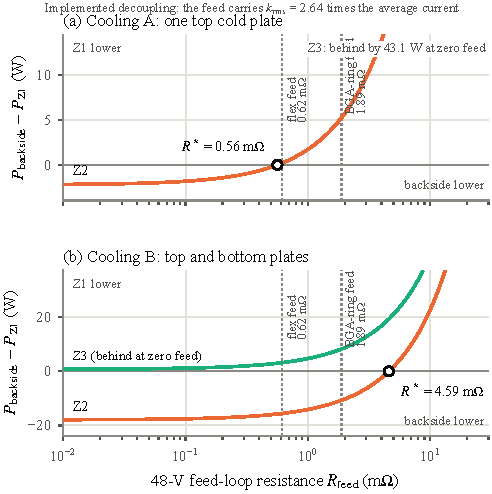
\includegraphics[width=\columnwidth]{fig6_crossover.pdf}
\caption{Platform-inclusive loss of the directly fed backside integrations minus that of Z1,
against the external feed-loop resistance. (a) S0. (b) S1. Below zero the backside integration
has the lower platform-inclusive loss; circles mark the crossover $R^*$. Dashed: the package
48-V loop resistance of Z1, for scale.}
\label{fig:feed}
\end{figure}

% ============================================================================ EXPLORE
\section{Exploring the Design Space}\label{sec:explore}

Exploration works at two levels. At the converter level the synthesis is repeated over the
regulator count and the topology (Section~\ref{sec:dse}, Fig.~\ref{fig:dse}): the optimum moves
to 76 cells with a two-branch topology, and a sweep with the topology held fixed misses it
because its feasible range ends at 52 cells. At the package level, every input without a single
defensible value is varied on the production mesh and the full chain is rerun, so that each
ranking of Section~\ref{sec:compare} is reported together with the decisions that can change
it. Fig.~\ref{fig:robust} summarizes \NvariantRuns{} such runs for the embedded and
package-backside pair at S0: for each decision and each ranking, whether the ranking is
preserved, withdrawn (the gap falls within twice its uncertainty) or reversed.

\begin{figure}[!t]
\centering
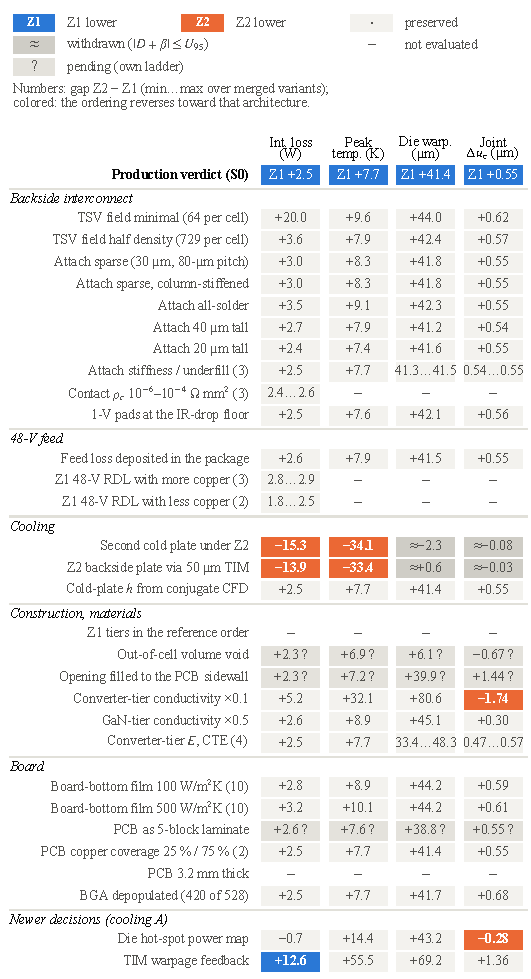
\includegraphics[width=\columnwidth]{fig9_robustness_map.pdf}
\caption{Ranking-robustness map, Z1 against Z2 at S0. Rows: package decisions varied on the
production mesh, grouped by the design choice they represent (merged rows give the number of
runs); columns: the rankings. Each cell shows whether the production ranking is preserved,
withdrawn (gap within twice its uncertainty) or reversed, with the architecture it then
favors.}
\label{fig:robust}
\end{figure}

% TODO(data): which decisions preserve / withdraw / reverse each ranking:
%  - tier order (z1_tier_reference): +x K, +y W -- realizability and electrothermal coupled
%  - backside cooling (z2_cooled): reverses the thermal and mechanical rankings?
%  - TSV provisioning (tsv_min), attach density (attach_sparse): electrical ranking
%  - out-of-cell construction (f2_void): mechanical ranking
%  - board boundary (board_hbot100/500): joint temperatures, calibration flags
%  - cooling model form (icepak_equivalent): peak temperature

% ============================================================================ DISCUSSION
\section{Discussion}\label{sec:discussion}

\subsection{Design rules from the coupled solution}
Each rule below follows from a result of Sections~\ref{sec:evaluate}--\ref{sec:explore} and is
invisible to the single-domain analysis that would normally make the decision.

\emph{Rank integrations on the converged electrothermal state.} The loss a regulator dissipates
depends on the temperature its integration imposes on it. At room temperature the
substrate-backside regulator is ahead of the embedded one by \DeltaPrtZtwoSzero~W and the
board-backside regulator behind it by \DeltaPrtAbsZthreeSzero~W; on the converged field the order
of each pair reverses, by \LossGapZtwoSzero~W and \LossGapZthreeSzero~W, because the converter's
thermal path changes its conversion loss by more than the routing changes. A placement study
that holds the converter loss fixed ranks the integrations in the wrong order.

\emph{An embedded regulator needs local input decoupling.} The package 48-V network of an
embedded regulator carries whatever waveform the cells draw. Without local input capacitance
the package loss rises by \RiseSoneZone~W and the critical joint leaves the calibrated range of
the solder law; with the input pulsed at the overall ratio there is no admissible operating
point. Directly fed backside regulators are insensitive to this choice.

\emph{Order the tiers for the interconnect technology.} With build-up microvias, the high-side
device, the flying capacitors, the low-side device and the inductors should be stacked in that
order: the reference order needs a via of aspect ratio 5.3, the repartitioned one 0.83, with the
same components, area and height. % TODO(data): + its electrothermal effect (z1_tier_reference)

\emph{A backside regulator needs a feed specification.} The direct 48-V feed is outside the
package and must be specified as a loop resistance below $R^*$; where the backside regulator is
behind at zero feed resistance, no connector recovers the difference.
% TODO(data): R* values

\emph{Size the package interface for the rail it carries.} Integrating the regulator on the
board backside removes the board opening, but sends the kiloampere 1-V current through the ball
field: at 1.5~A per ball it occupies 1334 of the 1369 sites of a 0.8-mm array, leaving almost no
signal balls, and only \LandBallsInside{} balls per rail lie under the cells. Redistributing
the rest laterally in the package land side costs \LandPmin--\LandPmax~W and
\LandDVmin--\LandDVmax~mV for \LandTmax--\LandTmin~\textmu m of copper. Keeping the 1-V
current under the cells requires a ball pitch of \PitchMaxZthree~mm or less.

\emph{Do not use temperature as a proxy for joint response.} The package-backside regulator
runs \dTmaxAbsZtwoSzero~K hotter at its peak than the embedded one, yet its critical joint is
\dTjointAbsZtwoSzero~K cooler, because the ball ring sits away from the converter; the joint
still moves \DuRatioZtwo{} times as far, because its driver is set by the bending of the plate the
balls support rather than by their temperature. A screen on joint temperature would rank the two
the wrong way round.

\subsection{Scope and limitations}
The framework is verified stage by stage against matched references, not against a measured
system; no fabricated DVPD package of this kind exists to measure. The converter loss model
omits core, alternating-current winding, dielectric and dead-time losses, which bias the
absolute loss downward by the same mechanism in every integration. The local solder response is
a per-cycle inelastic strain increment, not a life: no damage law or allowable is applied, and
the constitutive law is calibrated to 125\,$^\circ$C, so responses at hotter joints are flagged
as extrapolations. The mechanics is one-way coupled, which the small feedback of thermal strain on
resistance justifies in the intact regime but not for a damaged or delaminated interface. The board is a 30-mm coupon with a film beneath;
its lateral spreading is bracketed by the board-boundary sensitivity. The Z3 ledger omits the
board-plane and land-side 1-V redistribution and is therefore a lower bound, which the sheet
estimate above brackets. Every result belongs to one specification; the conclusions that
generalize are the mechanisms and rules, not the numbers.

% ============================================================================ CONCLUSION
\section{Conclusion}\label{sec:conclusion}

Integrating a voltage regulator at the point of load is not a placement choice that can be made
after the converter is designed: the integration sets the converter's temperature and therefore
its loss, the waveform its package interconnect carries, the deformation of the package and the
survival of the interconnect and ball-field rules. The framework presented here carries a
synthesized hybrid switched-capacitor--buck regulator through an explicit package to these
consequences on one geometry, verifies each stage against a matched reference, and does so in
\EvalHours{} per integration on a shared workstation. Used to evaluate, compare and explore, it showed on one 1-kW
specification that coupling reverses the electrical ranking of the integrations in both
directions, that the embedded regulator requires local input decoupling and a repartitioned tier
order, that the substrate-backside regulator warps the die \WarpRatioZtwo{} times as much as the
embedded one, that the board-backside regulator is limited by the ball field rather than by its
thermal or mechanical behavior, and that the regulator-count optimum shifts with the topology
chosen at each count.
The same chain applies to any member of the hybrid family, any package stack the builder can
express, and any cooling solution with a declared boundary, which makes it a design tool for the
integration decision itself rather than a check applied after it.


\bibliographystyle{IEEEtran}
\bibliography{refs}
\end{document}
